\documentclass{svmult} 

\RequirePackage{etex}
\usepackage[utf8]{inputenc}
\usepackage[english]{babel}
\usepackage{amsmath}
\usepackage{amssymb}
\usepackage{graphicx}
%\usepackage{url}
%\usepackage{color}
\usepackage{paralist} 
\usepackage{mathtools}
\usepackage{todonotes}
\usepackage{url}
%\usepackage{tikz}
%\usetikzlibrary{arrows,decorations.pathmorphing,backgrounds,positioning,fit,petri,matrix,automata,calendar,shapes,snakes,patterns}
%\usepackage{floatrow} 
%\usepackage{tabularx}
\usepackage{subfigure} 
%\usepackage{array} 
%\usepackage{booktabs} 
\usepackage{cleveref}
\usepackage[flushleft]{threeparttable}
%\usepackage{siunitx}
%\usepackage{setspace} 
%\usepackage{fullpage}
%\usepackage[left=4cm,right=4cm,top=1.5cm,bottom=1cm,includeheadfoot]{geometry}
 
\usepackage{color} % package für Schriftfarbe Verwenden:-> \textcolor{Farbe}{Text}
\newcommand{\MB}[2]{{\textcolor{gray}{#1}}\textcolor{blue}{#2}}
\newcommand{\TM}[2]{\textcolor{blue}{#2}}
\newcommand{\MM}[2]{\textcolor{orange}{#2}}
\newcommand{\m}[1]{\mathcal{#1}}

\begin{document}
\title*{Genome Rearrangement Analysis:}
\subtitle{Cut and Join Genome Rearrangements and Gene Cluster Preserving Approaches}
\author{Tom Hartmann, Martin Middendorf, Matthias Bernt}
 
\institute{Swarm Intelligence and Complex Systems Group, Institute of Computer
Science, University Leipzig, Germany, 
\email{{thartmann,middendorf,bernt}@informatik.uni-leipzig.de}
} 
\titlerunning{Genome Rearrangement Analysis}
\authorrunning{Hartmann et al.}

\abstract*{
Genome rearrangements are mutations that change the gene content of a genome or the arrangement of 
the genes on a genome. Several years of research on genome rearrangements have established 
different algorithmic approaches for solving some fundamental problems in comparative genomics 
based on gene order information.
This review summarizes the literature on genome rearrangement analysis along two lines of research. 
The first line considers rearrangement models that are particularly well suited for a theoretical analysis.
These models use rearrangement operations that cut chromosomes into
fragments and then join the fragments into new chromosomes.
The second line works with rearrangement models that reflect several
biologically motivated constraints, e.g., the constraint that gene
clusters have to be preserved. In this chapter, the border between algorithmically ``easy'' and ``hard'' rearrangement problems 
is sketched and a brief review is given on the available software tools for genome rearrangement analysis.
\keywords{gene order analysis, genome rearrangements, cut and join, gene
cluster}
}
\abstract{
Genome rearrangements are mutations that change the gene content of a genome or the arrangement of 
the genes on a genome. Several years of research on genome rearrangements have established 
different algorithmic approaches for solving some fundamental problems in comparative genomics 
based on gene order information.
This review summarizes the literature on genome rearrangement analysis along two lines of research. 
The first line considers rearrangement models that are particularly well suited for a theoretical analysis.
These models use rearrangement operations that cut chromosomes into
fragments and then join the fragments into new chromosomes.
The second line works with rearrangement models that reflect several
biologically motivated constraints, e.g., the constraint that gene
clusters have to be preserved. In this chapter, the border between algorithmically ``easy'' and ``hard'' rearrangement problems 
is sketched and a brief review is given on the available software tools for genome rearrangement analysis.
\keywords{gene order analysis, genome rearrangements, cut and join, gene
cluster}
}

\maketitle



\section{Introduction}

% General Genome rearrangement analysis. why what? 
During evolution the gene content as well as the arrangement of the genes within the genomes of species 
have been modified by various kinds of mutations. 
A genome consists of a set of chromosomes and each chromosome contains a set of genes. A chromosome represents 
a linear or circular string of DNA where the genes are located. Each gene of a chromosome has an orientation 
depending on which of the two strands of the DNA it is located. 
Mutations that change the arrangement of the genes on the
chromosome are called rearrangement mutations (or rearrangements). Examples are inversions that reverse the order and orientation 
of a subsequence of genes on a chromosome and transpositions 
which move a subsequence of genes from one chromosome to another location on the same or another chromosome.
Other examples are fissions which split a chromosome into two chromosomes and fusions which merge two chromosomes to form a 
single chromosome. In addition to such rearrangement mutations which do not change the gene content of a genome, there exist also 
rearrangements that change the gene content of a genome. However,
the latter type of rearrangements are not considered in this chapter.

Gene order analysis aims to explain the differences of the gene arrangement (and gene content) between the genomes of extant species 
and to reconstruct their phylogenetic evolution. The most common approach for
gene order analysis is maximum parsimony. This approach tries to explain the differences within a set of genomes by the minimum
possible number of changes. For example, on might ask for a shortest sequence of
(allowed) rearrangement mutations that transforms one given genome into another
given genome. This problem is called the sorting problem. The corresponding
problem that asks only for the smallest number of such mutations is called
distance problem. 
Such distance information between genomes of species can be used, e.g., to
reconstruct the phylogenetic relationships between the species, 
e.g.,~\cite{Wang_2006}.

%The thereby computed distances can be used for standard distance based
%reconstructions, e.g.,~\cite{Wang_2006}. 

% Computational Aspects and Problems 
The exploration of the combinatorial and computational problems that occur in gene order analysis started with the pioneering 
works of Sankoff and Blanchette~\cite{Sankoff_1992} and Watterson et al.~\cite{Watterson_1982}. Early breakthroughs have been 
obtained with respect to the sorting problem where polynomial time algorithms have been developed for the problem of sorting 
with inversions~\cite{Hannenhalli_1999} and for sorting with inversions plus fission and fusion~\cite{Hannenhalli_1995}. However, 
many other related problems have been shown to be NP-hard which makes it
unlikely that they can be solved optimally in polynomial time. Examples are the problem of sorting with inversions for unsigned 
genomes (i.e., the orientations of the genes are ignored)~\cite{Caprara_1997},
the inversion median problem (i.e., the problem to find a parsimonious common ancestral gene order for more than two given gene orders)~\cite{Caprara_2003}, 
and the problem of sorting by transpositions~\cite{Bulteau_2012}. Hence, one focus of the research in gene order 
analysis is to develop heuristics and approximation algorithms. Examples of such
algorithms are the frequently used \texttt{MGR} algorithm for solving the
inversion median problem~\cite{Bourque_2002} and approximation algorithms for the sorting by transpositions problem~\cite{Elias_2006}.

This chapter gives an overview on the different gene rearrangement problems and reviews the corresponding literature. 
We also give a brief review of the available software tools 
and web services for rearrangement analysis (see, e.g., \Cref{table:tools}).
The chapter is organized along two lines of research in gene order analysis. 

% Line of research: Cut and Join
The first line of research tries to find models of rearrangement mutations which are well suited for a theoretical analysis. 
These models are based on two operations: i) to cut a chromosome into fragments and ii) to rejoin such fragments (into new chromosomes). 
The differences between the models are the number of cut points of an operation and the different ways how the fragments can be rejoined. 
Thereby, most of the (classical) rearrangement operations are directly covered
and a few others, e.g., transpositions, can be emulated by a combination of such cut and join operations. One focus is to sketch the 
border between easy problems, i.e., problems that are polynomial time solvable and difficult problems, i.e., problems that are NP-hard.
 
% Line of research: constraints
The second line of research tries to identify biologically motivated constraints 
on the applicability of gene rearrangement mutations. One particular important
type of constraints are conserved gene clusters, i.e., subsets of the genes that are observed in close proximity on all given genomes. 
Such gene clusters might form due to functional constraints or evolutionary inertia. The idea is to consider such
conserved gene clusters in the reconstructions, i.e., genome rearrangement that break gene clusters are forbidden. 
Even if a rearrangement problem might become or remain NP-hard with such additional restrictions, e.g., the preserving 
inversion sorting problem~\cite{Figeac_2004}, the search space becomes more structured such that many problem instances 
can be solved efficiently~\cite{Berard_2007,Bernt_2009,Bernt_2007}.
It is worth to mention that in addition to the preservation of gene
clusters, other biologically motivated constraints have been introduced, e.g., positional constraints on gene 
adjacencies motivated on chromosome conformation information
\cite{Swenson_2016, Veron_2011}.


This chapter is organized as follows. In the next \Cref{Sec-Pre} a formal
background on gene arrangements and rearrangement mutations is given. In addition, the basic problems of gene order analysis are 
introduced. An overview on the literature on cut and join models of rearrangement mutations is presented in \Cref{sec:x-cut}. 
An overview on gene order analysis with conserved gene clusters is given in \Cref{sec:preserving_models}. 
The chapter ends with a conclusion in \Cref{Sec-Concl}.



% % Outline
% Here only/mainly same gene content 
% 
% 
% -Idea: most genome rrrmt problems are NP-hard which means that the
% calculation of exact solutions can not be done in reasonable time
% - thus one is limited to restrict genome rrrmt problems to guarantee their
% tractability
% -restrictions are usually done either used genome rrrmt model or additional
% constraint are used to give the search space a structure which can further be
% used to guide the solution construction
% - first : the challenge
% has been to find a consistent and biologically meaningful set of
% operations for which the genomic distance problem is still tractable.
% - examples for the first are: SBR,\ldots
% - examples for the latter are: perfect SBR, perfect TDRL median sorting, common
% intervals, 
% -idea is to approximate the real solution by different linear
% time computable algorithms for simplified problems
% \ldots
% 
% 
% - short summary of tool using different models? : DCJ: mauve,\ldots
% 
% - which problems we want to concentrate: problems in P/NP/open
% problems, present the ideas of the algorithms
% - also when the problems turn to be hard, e.g., sorting by inversions of signed
% and unsigned permutations
% - provide a state-of-art overview
% - dcj provides all events to model the process of excision, circularization,
% linearization and reincorporation which happens in the configuration of the
% immune respone of higher animals~\cite{Warren_2009}
% \todo[inline]{add sentence that we focus on problems where given genomes have
% the same set of genes without duplicates} 
% 
% The order of genes can changed during
% evolution and therefor a set of gene orders can provide information about there phylogenetic
% relationships.
% %
% A common method to find these relationships is to use different operations which
% can change the order of genes.
% %
% A model is formed by a set of operations and therefor a challenging problem is
% to find possible scenarios which transform one gene order into another.
% %
% 
% \todo{
% %%Motivation%%
% Based on great biological relevance in eukaryotic genomes a realistic model
% should include translocations, fusions, fissions, and inversions
%~\cite{Mazowita_2006,Yancopoulos_2005}.
% %
% The are also strong indications to include transpositions into a realistic model
%~\cite{Bergeron_2006b,Andersson_2000,Dalevi_2002,Kent_2003}.
% % 
% Due to computational intractabilities transpositions are less favoured
%~\cite{Bulteau_2012} while a generalization of transpositions called
% block-interchange~\cite{Christie_1996} preserves tractability.
% %
% A block-interchange allows the exchange of any two consecutive gene sequences in
% a genome.
% %
% In~\cite{Yancopoulos_2005} Yancopoulus et al. presented the \emph{double-cut
% and join}, or short $\m{DCJ}$, model which extents $\m{SCAJ}$ to include all the
% mentioned classical rearrangement events.
% }
% 
% 
% 
% %motivation for preserving model
% Solutions of genome rearrangement problems under unpreserving models do usually
% suffer from some biologically relevant problems.
% %
% Due to --in most cases-- exponential number of solutions~\cite{Bergeron_2002},
% e.g., scenarios of a sorting problem, it is challenging to determine one solution
% based on reliable arguments.
% %
% Further, the preservation of certain gene groups during evolution is
% already excepted. \re{CITE and EXAMPLES?} 
% %
% Especially for a large set of species which share specific gene groups 
% it seems to be acceptable that preservation of gene groups is attended by 
% %
% Current unpreserving approaches sometimes produce scenarios which break these
% gene groups~\cite{Berard_2004}.
% %
% Preserving genome rearrangement models overcome these limitations by satisfying
% the idea that ancestral genomes of species which show gene groups share this
% structure as well.
% %

\section{Preliminaries}
\label{Sec-Pre}

A formal background on gene arrangements, rearrangement mutations, and basic
problems of gene order analysis is given in this section.

\subsection{Gene Orders}
A \emph{genome} is a set of linear or circular DNA sequences which are called \emph{chromosomes}. 
Genomes are called \emph{unichromosomal} if they consist of only a single chromosome and \emph{multi\-chromosomal} otherwise. 
If all chromosomes of a genome are linear (resp. circular) then the genome is called \emph{linear} 
(resp. \emph{circular}) and \emph{mixed} otherwise. 

A \emph{gene} is a unit of genetic information that encodes a specific function. It is assumed here that each
gene has a unique identifier and that it can be identified whether a gene occurs in a 
genome or not. If a gene occurs in a genome it can be located and it corresponds to an 
oriented sequence of DNA. In this chapter we consider
only the case that genes within a genome do not intersect. If not stated otherwise, it is assumed that a gene 
occurs at most once in a genome. The set of genes of a genome $\alpha$ is denoted by $\mathcal{G}(\alpha)$.
A gene $g$ can be represented by its \emph{extremities}: the \emph{tail}
$g^t$ and the \emph{head} $g^h$, i.e., the 5' and 3' end of the gene. A linear (resp. circular) 
chromosome can be represented by the linear (resp. circular) sequence of the extremities of its genes. 
% The set of all extremities of the genes of a genome $G$ is denoted by 
% $\mathcal{E}(G)$, i.e., $\mathcal{E}(G)= \{ x^h,x^t: x \in \mathcal{G}(G)\}$.
%
%%%% paralogous genes definitions %%%%
% In the case that DNA contains copies of paralogous genes which are called
% \emph{paralogs}, the extremities are arbitrarily assigned to a subscript.
% %
% Thus by $g_1^t,g_1^h,g_2^t$, and $g_2^h$ we denoted the paralog extremities of a
% dulpicated gene $g$.
% %
% Given an extremity $x$ we denote the paralog extremity with $\hat{x}$, e.g.,
% for $x_1^t$ the equation $\hat{x}_1^t=x_2^t$ is satisfied.
% %

%adjacency
Given a genome $\alpha$, an \emph{adjacency} is an unordered pair $\{p,q\}$ of
extremities $p$ and $q$, $p\neq q$, of genes of $\mathcal{G}(\alpha)$ that are
adjacent on a chromosome of $\alpha$. The endpoints of linear
chromosomes are called \emph{telomeres}.
A telomere is denoted by the pair $\{p,\circ\}$, where $p$ is the
extremity that is closest to the telomere and therefore $p$ is not adjacent to the extremity of another gene.
The set of all telomeres of a genome $\alpha$ is denoted by
$\mathcal{T}(\alpha)$.
The set of extremities $\mathcal{E}(\alpha)$ of a genome $\alpha$ consists of
all extremities of the genes, i.e., $\mathcal{E}(\alpha)= \{
g^h,g^t: g \in \mathcal{G}(\alpha)\}$.
%genome
A genome $\alpha$ can be characterized by the set of adjacencies of its genes 
and its telomeres, for simplicity let $\alpha$ denotes this set.
%
Furthermore, $\mathcal{I}(\alpha)$ denoted the set of all adjacencies (without
the telomeres) of a genome, i.e.,
$\mathcal{I}(\alpha)=\alpha\setminus\mathcal{T}(\alpha)$.
Note that $\mathcal{I}(\alpha)$ uniquely determines the set of telomeres.
%
For a set of genes $\mathcal{G}$, the set of all possible genomes is denoted by $\mathbb{G}(\mathcal{G})$ (or simply 
$\mathbb{G}$ if the context is clear). 
%

%% previously needed for definition of common intervals, I do not need it, do I?
% Given a set of genes $\mathcal{G}$ and a genome $G$ with $G_{|\mathcal{G}}$ the
% subset of adjacencies of $G$ which only contain extremities of $\mathcal{G}$ is
% denoted, i.e., an adjacency $\{p,q\} \in G$ is contained in $G_{|\mathcal{G}}$
% if and only if $p,q \in \mathcal{E}(\mathcal{G})$.
%chromosome
A genome $\alpha$ can be represented by an undirected graph -- the \emph{genome graph} -- which contains the
extremities as vertices and an edge connects two vertices $x$ and $y$ if and
only if either $\{x,y\}$ is an adjacency in $\alpha$ or $x$ and $y$ are head and tail of the same gene.
\emph{Linear} and \emph{circular} chromosomes correspond to linear and 
circular connected components in the genome graph. 
\Cref{fig:genome_graph} illustrates an example of a genome graph.
%

A \emph{weighted genome graph} $wGG$ is a genome graph that has a nonnegative integer
weight for each edge that connects two extremities $x$ and $y$ if and only if either
$\{x, y\}$ is an adjacency or one of $x$, $y$ is a telomere. The weight $w(\alpha)$ of a
genome $\alpha$ is the sum of the weights of all edges of $wGG(\alpha)$.  

\begin{figure}
	\centering
	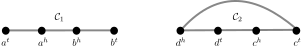
\includegraphics[width=.65\textwidth]{figures/genome_graph_example.pdf}
	\caption{Genome graph of the mixed multichromosomal genome
	$\alpha=\{\{a^t,\circ\},\{a^h,b^h\},\{b^t,\circ\},
	\{c^t,d^h\},\{d^t,c^h\}\}$ consisting of the linear chromosome
	$\mathcal{C}_1=\{\{a^t,\circ\},\{a^h,b^h\},\{b^t,\circ\}\}$ 
	and the circular chromosome $\mathcal{C}_2=\{\{c^t,d^h\},\{d^t,c^h\}\}$.
	The set of telomeres of $\alpha$ is
	$\mathcal{T}(\alpha)=\{\{a^t,\circ\},\{b^t,\circ\}\}$.
	Genome $\alpha$ can also be represented by $S_\alpha=\{
	(a~-{b}),(-{d}~-{c})^\circ\}$, where $^\circ$ marks the chromosome as
	circular.}
	\label{fig:genome_graph}
\end{figure}

An alternative representation of a genome $\alpha$ is a set of signed strings
$S_{\alpha}$, where each string lists the genes of one chromosome as if 
read from one telomere to the other (or in the case of circular chromosomes
starting from an arbitrary gene), see \Cref{fig:genome_graph}. 
If the head of a gene $x$ appears before its tail the gene in the string
gets a negative sign (represented by $-{x}$), otherwise a positive
sign is assigned to the gene (a positive sign is omitted).
The sign represents the (relative) strandedness of the genes. 
Both strings of the two reading directions of a linear
chromosome and also all strings generated from different start points in circular chromosomes are considered to be equivalent.
Note, that for some applications this assumption might not be useful, e.g. if parts chromosomes with known orientation.
For unichromosomal genomes with $n$ genes
this representation is equivalent to a \emph{signed permutation} of length
$n$. Such a permutation $\pi$ is denoted by
$(\pi(1)~\pi(2)\ldots\pi(n))$, where $\pi(i)$ denotes the $i$-th element.
The identity permutation $(1~2\ldots ~n)$ is denoted by $\iota$.
For differentiation the string corresponding to a circular chromosome is enclosed between $()^\circ$.
In the following the two representations of unichromosomal genomes are
used interchangeably, where $\pi$ and $\sigma$ denote genomes as permutations,
and $\alpha$ and $\beta$ denote genomes as sets of adjacencies and telomeres.
The considered genomes are always assumed to consist of the same
set of genes throughout this chapter.

% definition common intervals 
Often in nature a subset of genes is found in close proximity in the genomes 
of many different species. Such a set of genes is called gene
cluster~\cite{Graham_1995}.
A simple formal model for gene clusters are \emph{common intervals}~\cite{Heber_2001}. An \emph{interval} 
$I$ of a permutation $\pi$ of length $n$ is a subset of elements of $\pi$ which form a consecutive segment, i.e., 
there exists a pair $(i,j)$, with $1 \leq i \le j \leq n$, such that
$\{|\pi(x)|:
i\leq x \leq j\}=I$.
For a set of signed permutations $\Pi$ a common interval is a subset of the elements of the permutations that 
is an interval in each permutation in $\Pi$. Singleton sets $\{i\}$ with $i\in[1:n]$ as well as $\{1,\ldots,n\}$ 
are called \emph{trivial common intervals}.
The set of all common intervals of a set of permutations $\Pi$ is denoted by
$C(\Pi)$.
A set of permutations $\Sigma$ is \emph{consistent} with the common intervals
of a set of permutations $\Pi$ if $C(\Pi)=C(\Pi \cup \Sigma)$.

\subsection{Rearrangement Model}


Different types of rearrangement mutations are of interest for rearrangement analysis. See \Cref{fig:events} for a selection of such rearrangement mutations. The set of possible rearrangement mutations that is of interest is called a rearrangement model. 

\begin{figure}
	\begin{center}
	\subfigure[inversion]{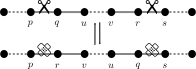
\includegraphics[width=.38\textwidth]{figures/event_inversion.pdf}}
	\quad
	\subfigure[block interchange]{
	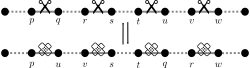
\includegraphics[width=.49\textwidth]{figures/event_block_interchange.pdf}}
	\subfigure[fusion/fission]{\includegraphics[width=.38\textwidth]{figures/event_fusion_fission.pdf}}
	\quad
	\subfigure[translocation]{\includegraphics[width=.49\textwidth]{figures/event_translocation.pdf}}
	\end{center}
	\caption{Rearrangement events visualized on the genome graph. (a) An inversion reverses the order of the 
	genes between two cut points (a cut is indicated by a scissor, a join is
	indicated by a plaster) and inverses the orientation of the affected genes. (b) A block interchange swaps two intervals. If the two intervals are 
	adjacent, i.e., the middle cut points coincide, it is a transposition. (c) A fission cuts out an interval and 
	creates a circular chromosome. 
	A fusion inverts this operation. (d) A translocation swaps the ends of two chromosomes. }
	\label{fig:events}
\end{figure}
% \begin{figure}
% 		\centering
% 		
\includegraphics[width=.6\textwidth]{figures/rev_model_example.pdf}
% 		\caption{An event $(\alpha,\alpha')\in \m{INV}$.
% 		Adjacencies that are cut or joined by the event are marked by 
% 		scissors or a plaster, respectively. Dotted lines indicate
% 		additional adjacencies. Note that the order of the genes
% 		between the extremities $q$ and $r$ is reversed by the event.
% 		Since an inversion is a symmetric event the scissors and
% 		plasters can be exchanged.}
% 		\label{fig:rev_example}
% \end{figure}

Along the lines of~\cite{Bergeron_2010} a \emph{rearrangement model}
$\mathcal{M}$ is defined as a binary relation over the set of all possible
genomes, i.e., $\mathcal{M} \subseteq \mathbb{G} \times \mathbb{G}$.
%
A pair of genomes $\mathcal{R}=(\alpha,\alpha')$ is a \emph{rearrangement event}
in $\mathcal{M}$ if and only if $\mathcal{R} \in \mathcal{M}$. The event $\mathcal{R}$ can be considered as a rearrangement that
transforms $\alpha$ into $\alpha'$, we write $\alpha'=\alpha \circ \mathcal{R}$.
%
%scenario
Given two genomes $\alpha$ and $\alpha'$ and a (rearrangement) model
$\mathcal{M}$, a \emph{scenario} is a sequence $\mathcal{R}_1,\ldots,
\mathcal{R}_k$ of rearrangement events in $\mathcal{M}$ with
$\alpha'=\alpha \circ \mathcal{R}_1\circ\ldots\circ\mathcal{R}_k$.
The set of all possible scenarios for two given
genomes $\alpha$ and $\alpha'$ is denoted by $\mathcal{S}_\mathcal{M}(\alpha,\alpha')$.
% rearranging genome $G_1$ into genome $G_2$ under $\mathcal{M}$ is a subset
% $S^\mathcal{M}_{(G_1,G_2)}$ of $\mathcal{M}$ such that for all $(G_i,G_j)\in
% S^\mathcal{M}_{(G_1,G_2)}$ one of the following conditions holds:
% \begin{inparaenum}[i)]
% 	\item There exist $(G_h,G_i) \in S^\mathcal{M}_{(G_1,G_2)}$ and $(G_j,G_k)
% 	\in S^\mathcal{M}_{(G_1,G_2)}$.
% 	\item There exist $(G_1,G_j) \in S^\mathcal{M}_{(G_1,G_2)}$ or
% 	$(G_i,G_2) \in S^\mathcal{M}_{(G_1,G_2)}$.
% \end{inparaenum}
The most famous rearrangement model for unichromosomal genomes is the inversion 
-- or reversal -- model ($\mathcal{INV}$). This model consists of all inversion operations 
and was studied first in~\cite{Sankoff_1992,Watterson_1982}. 
% An inversion reverses the order of the genes in an interval of a gene order and switches the sign of every contained element, see \Cref{fig:events}~(a). 
% %
% In the definition of signed permutations an \emph{inversion} $\rho$ applied to
% a permutation $\pi$, denoted by $\pi\circ\rho$, is a rearrangement operation
% which reverses a continues sequence of genes and inverts the sign of every
% affected gene.
% See \Cref{fig:events} for other important rearrangement operations.


%%%%%% preserving definition %%%%%%
For each rearrangement model $\mathcal{M}$ a corresponding preserving
variant, denoted by $\m{M}^p$, can be defined as the set of
rearrangement operations of $\m{M}$ which do not destroy any common interval of
the two given gene orders in any of its intermediate gene orders. 
Formally, an event $\rho=(\pi,\pi')$ of a model $\m{M}$ is called \emph{preserving} with 
respect to a set of permutations $\Pi$ if $C(\Pi)=C(\Pi \cup \{\pi,\pi'\})$, i.e., $\pi$ as well as $\pi'$ are consistent with $\Pi$. 
% , i.e.
% %
% The preserving variant of $\m{M}$ is defined as $\m{M}^p = \{(\pi,\pi')\in \m{M} : C(\Pi\cup \{\pi,\pi'\} \}$. 

\subsection{Genome Rearrangement Analysis}

There exist several approaches to extract phylogenetic information from 
gene arrangement data, see \cite{Felsenstein_2004} for a comprehensive
overview. One example is the computation of rearrangement distances between genomes. Another example is the
joint reconstruction of a phylogenetic tree for a set of genomes and the corresponding rearrangement events along its edges. 
In the following the central 
combinatorial problems that need to be solved for such approaches are formally defined.

% distance
% Assume a model $\mathcal{M}$ and two genomes $\alpha$ and $\alpha'$ on the same
% set of genes (which is assumed throughout the chapter).
Given a rearrangement model $\mathcal{M}$ and two genomes $\alpha$ and $\alpha'$ the 
\emph{distance problem} for $\mathcal{M}$ is to find the minimum number 
$d_\mathcal{M}(\alpha,\alpha')$ of events from $\mathcal{M}$ to transform
$\alpha$ into $\alpha'$. That is,
$d_\mathcal{M}(\alpha,\alpha')=\min_{S\in\mathcal{S}_\mathcal{M}(\alpha,\alpha')}|S|$.
To find a corresponding reconstruction, i.e., a corresponding scenario that transforms one genome into 
the other is called \emph{sorting problem}. The name is motivated by the fact that, 
by relabeling the elements of $\alpha$ and $\alpha'$, we can always assume that $\alpha'$ is the identity
permutation $\iota$. 
%
For a rearrangement model $\mathcal{M}$ that includes events which involve a
constant number of cuts it holds that for every $\alpha\in\mathbb{G}$ the set 
$\{ (\alpha,\alpha')\in \mathcal{M} : \alpha'\in\mathbb{G} \}$ has
polynomial size. This are in particular all models involving a subset of the
rearrangement operations that are shown in \Cref{fig:events}. 
For such models it holds that the sorting problem can be solved 
in polynomial time if a polynomial time algorithm solves the distance problem, e.g.,~\cite{Bergeron_2010,Hannenhalli_1999}.
% In general, it holds for a model $\mathcal{M}$ that the sorting problem can be solved 
% in polynomial time if a polynomial algorithm solves the distance problem since
% for every $\alpha\in\mathbb{G}$ it holds that $|\{ (\alpha,\alpha')\in
% \mathcal{M} : \alpha'\in\mathbb{G} \}|$ has polynomial size, see also
%~\cite{Bergeron_2010,Hannenhalli_1999}.
Due to the close connection between the sorting problem and the distance problem this chapter is focused on the distance problem. 
However, the sorting problem can sometimes be solved faster than by testing all possible rearrangement events, e.g., the sorting problem 
for the $\m{INV}$ model can be solved in sub-quadratic time~\cite{Tannier_2004}. It should be mentioned that the distance problem 
was studied for the first time in~\cite{Sankoff_1992} for the case of the $\m{INV}$ model.
In~\cite{Hannenhalli_1999} a polynomial time algorithm for
the sorting problem of signed permutations was given for the $\m{INV}$ model.
Examples of software tools which can solve this problem are \texttt{SORT$^2$},
\texttt{UniMoG}, and \texttt{baobabLUNA}. In addition, the software tool
\texttt{revDis} can be used to solve the distance problem under $\m{INV}$.
See \Cref{table:tools} for a summary.

Two central problems of gene order analysis for more than two genomes are the 
small and the large parsimony problem for gene orders. 
% small parsimony problem
The \emph{small parsimony problem} for a rearrangement model $\m{M}$ and a given
binary tree $T$ where every leaf is associated to a genome asks for one ancestral genome $\alpha_{i}$ for every inner vertex $i$ of 
$T$ such that the sum of the distances between the two genomes of an edge of the
tree is minimized, i.e., $\sum_{(u,v)\in E(T)}d_{\m{M}}(\alpha_u,\alpha_v)$ has to be minimized, where $E(T)$ is the set of edges of $T$.
% big parsimony problem
For the \emph{large parsimony problem} (also known as multiple genome rearrangement problem) the tree itself is sought in addition to the ancestral
genomes at its inner vertices. The small and the large parsimony problem for gene orders were both studied, e.g., 
in~\cite{Sankoff_1998}.

%median
A special case of the parsimony problems for rearrangement model $\m{M}$ is the \emph{median problem} which asks for a gene order 
$\alpha$ that minimizes the sum of the distances to given genomes $\alpha_1,\ldots,\alpha_k$, i.e., to find a $\alpha$ 
with $\min_{\alpha \in \mathbb{G}} \sum_{i=1}^{k}d_{\m{M}}(\alpha,\alpha_i)$.
%Note, that is this case the tree has only one inner vertex.
Mostly, the case of $k=3$ is considered. The solution of this case is often used in algorithms for solving larger multiple
genome rearrangement problems~\cite{Bourque_2002,Moret_2001,Zhang_2009}.
%
With a few notable exceptions~\cite{Feijao_2011,Ohlebusch_2007,Tannier_2009} the
small parsimony problem has been proven to be NP-hard for most rearrangement
models. For example, the median problem with $k=3$ is NP-hard for inversions~\cite{Caprara_1997} 
and for transpositions~\cite{Bader_2011}. However, the software tools
\texttt{median} and \texttt{GRAPPA} provide solver for both of these problems,
see \Cref{table:tools}.

Genome rearrangement problems that are defined for preserving rearrangement models are called \emph{preserving genome rearrangement problems}. 
For a discussion of further rearrangement models and problems see~\cite{Fertin_2009}.
In the following sections several basic algorithms for rearrangement models with and without the preserving property are studied. 

\begin{table}
\caption{List of resources and web services which are thematically related;
sorting problem (SP), distance problem (DP), median problem (MP), small parsimony problem (SPP), large parsimony problem
(LPP), transpositions ($\m{TR}$), inverse transpositions ($\m{ITR}$), model including
inversions, translocations, fusions, and fissions ($\m{HP}$), duplications and deletions
($\m{IND}$), block-interchanges ($\m{BI}$), restricted $\m{DCJ}$ events
($\m{RDCJ}$), tandem-duplications ($\m{TD}$), duplications ($\m{D}$), weighted
inversions ($\m{WINV}$).}
\begin{center}
\begin{threeparttable}
  \begin{tabular}{l l p{7.2cm}}
    \hline
    Resource & Reference & Features/Note\\
    \hline \\
    Web services & & \\
    \hline
    \texttt{CEGeD} & \cite{CEGeD,Bergeron_2006} & DP under
    $\m{INV}$, $\m{TR}$, and $\m{DCJ}$\\
    \texttt{CREx} & \cite{CREX,Bernt_2007b} & SP under
    $\m{INV}^p\cup\m{TR}^p\cup\m{ITR}^p$ and TDRL \\
    \texttt{GEvolutionS} & \cite{GEvolutionS} & simulates scenarios under
    $\m{TR}\cup\m{DCJ}\cup\m{HP}$\\
    \texttt{GRIMM}\tnote{a} & \cite{Tesler_2002b,GRIMM} & SP under $\m{HP}$ and $\m{INV}$ \\
    \texttt{MGR}\tnote{a} & \cite{MGR,Bourque_2002} & LPP under $\m{INV}$
    and $\m{HP}$\\
    \texttt{MGRA} & \cite{Alekseyev_2009,MGRA} & SPP and LPP under $\m{DCJ}$\\
    \texttt{MLGO} & \cite{MLGO,Hu_2014} & SPP and LPP under $\m{DCJ}\cup\m{IND}$\\
    \texttt{Roci} & \cite{Stoye_2009,ROCI} & SPP including
    $\m{INV} \cup \m{TR} \cup \m{ITR}$ while preserving conserved intervals\\
    \texttt{SORT$^2$} & \cite{SORT2,Huang_2010} & SP under $\m{INV}$,
    $\m{BI}$, $\m{HP}\cup\m{BI}$, and $\m{INV}\cup\m{BI}$; infers
    phylogenetic trees based on distances \\
    \texttt{SBBI}\tnote{a} & \cite{Christie_1996,SBBI} & SP under $\m{BI}$\\
    \texttt{UniMoG}\tnote{a} & \cite{UniMoG} & DP and SP under
    $\m{RDCJ}$, $\m{INV}$, $\m{TR}$, and $\m{HP}$     \vspace{0.2cm}\\
    Software for download & & \\
    \hline
    \texttt{baobabLUNA} & \cite{baobabLUNA,Braga_2009b}& DP and SP under $\m{INV}$; builds breakpoint
    graphs\\
    \texttt{dcjdDist} & \cite{DCJDDIST,Bader_2009} &  phylogenetic
    reconstruction under $\m{INV}\cup\m{BI}\cup\m{TD}\cup\m{D}$\\
    \texttt{DING} & \cite{DING,bohnenkaemper2021naturalgenomes} & DP under $\m{DCJ}\cup\m{IND}$\\
    \texttt{EMRAE} & \cite{EMRAE,Zhao_2009} & LPP for synteny blocks
    under $\m{INV}\cup\m{HP}\cup\m{TR}$ \\
    \texttt{GENESIS} & \cite{Gog_2008,GENESIS} & SP under
   	 $\m{WINV}$, $\m{WINV}\cup\m{TR}$, $\m{WINV}\cup\m{HP}$, and
    $\m{WINV}\cup \m{HP} \cup \m{TR}$\\
    \texttt{GRAPPA} & \cite{GRAPPA,Moret_2001}& LPP under $\m{INV}$\\
    \texttt{GREDU} & \cite{GREDU,Shao_2014} & DP under
    $\m{DCJ}\cup\m{IND}$\\
    \texttt{Mauve} & \cite{Darling_2004,Mauve}& multiple alignment tool; 
    DP of synteny blocks under $\m{DCJ}$ \\
    \texttt{median} & \cite{Bader_2008,PHYLO}\tnote{b} &
    MP under $\m{INV}$, $\m{TR}$, and $\m{WINV}\cup\m{TR}$\\
    \texttt{minswrt} &
    \cite{Bader_2008,PHYLO}\tnote{b} & DP under $\m{WINV}\cup\m{TR}$\\
    \texttt{MSOAR} & \cite{Zheng_2007,MSOAR}& calculates orthologous
    genes of genomic sequences involving genome rearrangements ($\m{HP}\cup
    \m{IND}$) \\
    \texttt{PATHGROUPS} & \cite{Zheng_2011,Pathgroups} & SPP under $\m{DCJ}$\\
    \texttt{phylo} & \cite{Bader_2008,PHYLO} & phylogenetic
    reconstruction under  $\m{WINV}\cup\m{TR}$\\
    \texttt{revDis} & \cite{Bader_2008,PHYLO}\tnote{b} & DP
    under $\m{INV}$ \\
    \texttt{weightedbb} & \cite{Bader_2008,PHYLO}\tnote{b} & branch and
    bound algorithm for DP under $\m{WINV}\cup\m{TR}$\\
    \hline
  \end{tabular}
  \label{table:tools}
  \begin{tablenotes}
    \item[a] Also available for download and local use.
    \item[b] And included references.
\end{tablenotes}
\end{threeparttable}
\end{center}
\end{table}


\section{Cut and Join Genome Rearrangement Models}
\label{sec:x-cut}
%
This section reviews results for unconstrained rearrangement analysis, i.e., 
without additional constraints, e.g., to preserve gene cluster. The focus is on the so-called \emph{cut and/or join} models. 
In particular, these are the single-cut or join model, the single-cut and join model, the double-cut and join model, and the multi-cut 
and join model.
%
Since many of the results are based on particular graph structures these are 
introduced first in the following subsection.

\subsection{Genome Rearrangement Graphs}

%breakpoint graph
The \emph{breakpoint graph} for signed genomes is a key element of efficient
algorithms for the calculation of the distance between genomes under the
$\m{INV}$ model~\cite{Hannenhalli_1999}.
%
For a source genome $\alpha$ and a target genome $\alpha'$ the breakpoint graph
$BP(\alpha,\alpha') = G(V,E_b \cup E_g)$ is defined as follows (see also 
\Cref{fig:breakpoint_graph_circular}). The vertices correspond to the
extremities of the genes, i.e., $V=\m{E}(\alpha)$. \emph{Black edges} connect
adjacent extremities of the source genome, i.e., $E_b=\alpha$ and \emph{gray edges} connect adjacent extremities of the target
genome, i.e., $E_g=\alpha'$.


%
For linear genomes two auxiliary vertices are added that are assumed to be
adjacent to the first, respectively, the last extremity of the two genomes.
Since each vertex has degree two the breakpoint graph can be 
partitioned into cycles, each of them with alternating black and gray edges. 
%
If both genomes are equal the breakpoint graph consists of a partition into color-alternating cycles of length two. 
Such cycles are called \emph{one-cycles}.
%
An extension of the breakpoint graph for more than two genomes has been
introduced in~\cite{Caprara_2003} to solve the median problem for $\m{INV}$.
%
The software tool \texttt{baobabLUNA} provides a function which builds the
breakpoint graph for two given genomes, see \Cref{table:tools}.

\begin{figure}
\centering
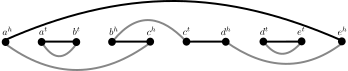
\includegraphics[width=.7\textwidth]{figures/breakpoint_graph_circular.pdf}
\caption{Breakpoint graph for the circular genomes
$S_{\alpha}=\{(-{a}~b~-{c}~-{d}~e)^\circ\}$ and
$S_{\alpha'}=\{(a~-{c}~-{b})^\circ,(-{d}~e)^\circ\}$. Adjacencies of
$\alpha$ (resp. $\alpha'$) are represented by black (resp. gray) edges. Note that the
edges of $BP(\alpha,\alpha')$ form a partition into alternating cycles and 
adjacencies that are common to both genomes form one-cycles.}
\label{fig:breakpoint_graph_circular}
\end{figure}

%adjacency graph
The \emph{adjacency graph} $AG(\alpha,\alpha')$ is the line graph of the
breakpoint graph of two genomes $\alpha$ and $\alpha'$ \cite{Bergeron_2006},
see \Cref{fig:adjacency_graph_circular}.
%
Hence, the vertices of the adjacency graph are the adjacencies and telomeres 
of both genomes and edges connect two adjacencies if and
only if they share one extremity, i.e., the edge multi set is given by $\{\{u,v\} : u\in\alpha, v\in\alpha', u\cap v\neq \emptyset \}$.
% Note that this definition leads to exactly two edges
% between two vertices corresponding to the different genomes when the vertices have the same adjacency.
As for the breakpoint graph, shared adjacencies form cycles of
the length two. But in contrast to the breakpoint graph, these cycles consists
of color alternating vertices instead of color alternating edges. Since this is
only a cosmetic difference, both cycles of length two are referred as
one-cycles.
% To visualize the duality of the breakpoint graph and the adjacency graph by
% the usage of a so-called \emph{master graph} the reader is encouraged to see
%~\cite{Friedberg_2008}.
%
The degree of a vertex is one if it is a telomere and two otherwise. Since the
adjacency graph is bipartite every cycle has an even length.
%
Hence, the adjacency graph consists of cycles, \emph{even paths}
which connect telomeres of the same genome, and \emph{odd paths}
which connect telomeres of different genomes.
%
% The number of even paths and odd paths of a given adjacency graph is denoted
% by $E$ and $I$, respectively.
%
An even path which starts and ends at an adjacency that belongs to the same
genome $\alpha$ is called \emph{$\alpha$-path}.
%
% Since the adjacency graph is
% dual to the breakpoint graph, edges in the breakpoint graph represent
% vertices in the adjacency graph and vertices in the breakpoint graph represent
% edges in the adjacency graph.
%
% This is illustrated by gray vertices of lower vertices which represent
% gray edges of \Cref{fig:breakpoint_graph_circular} and upper black vertices
% representing black edges of the breakpoint graph illustrated in \Cref{fig:breakpoint_graph_circular}.

\begin{figure}
	\centering
	\subfigure[]{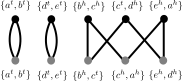
\includegraphics[width=0.35\textwidth]{figures/adjacency_graph_circular_changed_color.pdf}}
	\quad
	\subfigure[]{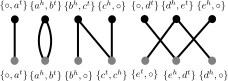
\includegraphics[width=0.44\textwidth]{figures/adjacency_graph_mixed.pdf}}
	\caption{(a) Adjacency graph for the circular genomes of
	\Cref{fig:breakpoint_graph_circular}. The adjacency graph contains three
	cycles. To visualize that 
	$AG(\alpha,\alpha')$ is the line graph of $BP(\alpha,\alpha')$ gray (resp.
	black) vertices of $AG(\alpha,\alpha')$ correspond to gray (resp. black) edges
	of $BP(\alpha,\alpha')$ and the edges of $AG(\alpha,\alpha')$ correspond to the
	vertices of $BP(\alpha,\alpha')$.
	(b) Adjacency graph for mixed genomes $S_{\beta}=\{(a~b~c),(d~e)\}$ and
	$S_{\beta'}=\{(-{b}~-{a}),(c)^\circ,(e~d)\}$.
	$AG(\beta,\beta')$ consists of one cycle, two odd paths, and two even
	paths.}
	\label{fig:adjacency_graph_circular}
\end{figure}

The breakpoint graph and the adjacency graph can both be constructed in linear time and require linear space~\cite{Bergeron_2006}. 
%
The adjacency graph has the potential advantage that the genes of the two genomes are separated whereas they are tangled 
in the breakpoint graph which complicates the interpretation~\cite{Friedberg_2008}. 

\subsection{Single-Cut or Join Model}
\label{sec:scoj}

The \emph{single-cut or join} model $\m{SCOJ}$~\cite{Feijao_2011}
includes two types of rearrangements (see \Cref{fig:SCOJ_events}): A \emph{cut} breaks an adjacency which creates two telomeres 
and a \emph{join} forms a new adjacency by connecting two telomeres. 
%
Formally, a pair of genomes $(\alpha,\alpha')$ is in
$\m{SCOJ}$ if and only if there exist different extremities $p$ and $q$ such that 
either $\alpha \cup \{\{p,\circ\},\{\circ,q\}\}=\alpha' \cup \{p,q\}$ (cut) or $\alpha
\cup \{p,q\} =\alpha' \cup \{\{p,\circ\},\{\circ,q\}\}$ (join) holds.
The single-cut or join model is a simplistic approximation of genome
rearrangement evolution since all genome rearrangements can be
represented by compositions of cuts and joins. 
However, this model has the advantage to allow for an efficient solution of some core problems of 
genome rearrangement analysis as explained in the following. 
More realistic models are described in the next sections.

\begin{figure}
\centering
\subfigure[]{\raisebox{.5cm}{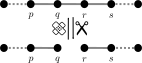
\includegraphics[width=0.3\textwidth]{figures/scoj_genome_graph.pdf}}\label{fig:SCOJ_events}}\quad
\subfigure[]{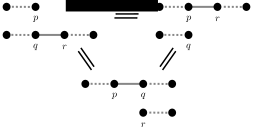
\includegraphics[width=0.5\textwidth]{figures/scaj_genome_graph.pdf}\label{fig:SCAJ_events}}
\caption{Genome graphs representing rearrangement events. Dots indicate the existence of additional edges. \subref{fig:SCOJ_events} Events of the $\m{SCOJ}$ model: cut event and join event. \subref{fig:SCAJ_events}
	Cut-and-join event of the $\mathcal{SCAJ}$ model. Together, both figures
	display the events of the $\mathcal{SCAJ}$ model.
}\label{fig:SCAOJ_events}
\end{figure}

\paragraph{Polynomial Time Solvable Problems}

For the $\mathcal{SCOJ}$ model efficient algorithms are known for the distance
problem, the sorting problem, the median problem, and the small parsimony
problem~\cite{Feijao_2011}.

%distance problem
Under $\mathcal{SCOJ}$ a parsimonious scenario for two genomes $\alpha$ and
$\alpha'$ is obtained by cutting all adjacencies which are in $\alpha$ but not
in $\alpha'$ and joining all extremities which are in $\alpha'$ but not in
$\alpha$.
Hence, $d_{\mathcal{SCOJ}}(\alpha,\alpha')=|\mathcal{I}(\alpha) \triangle \mathcal{I}(\alpha')|$ 
where $\triangle$ denotes the symmetric difference,
i.e., for two sets $X$ and $Y$ it holds $X \triangle Y:=(X\setminus Y)\cup(Y
\setminus X)$.

This also solves the sorting problem under $\m{SCOJ}$ in
linear time. For details see~\cite{Feijao_2009}.
The distance $d_{\mathcal{SCOJ}}(\alpha,\alpha')$ can also be interpreted 
in terms of the adjacency graph $AG(\alpha,\alpha')$.
It holds that $d_{\mathcal{SCOJ}}(\alpha,\alpha')=2N-2C_2-P$, where $N$ is the
number of genes, $C_2$ is the number of one-cycles, and $P$ is the
number of paths in $AG(\alpha,\alpha')$. 
This is because 
$|\mathcal{I}(\alpha)|=N-t_\alpha/2$, where $t_\alpha$ is the number of
telomeres of $\alpha$ (analogously this holds for $\alpha'$), $|\mathcal{I}(\alpha)\cap \mathcal{I}(\alpha')|=C_2$ and the
fact that a path always connects two telomeres.
% The correctness of the formula can be verified by
% $d_{\mathcal{SCOJ}}(G,G')=|G^\circ \setminus G'^\circ|+|G'^\circ \setminus G^\circ|= |G^\circ| + |G'^\circ| - 2|G^\circ \cap G'^\circ|$.

%median problem
The median problem under $\mathcal{SCOJ}$ can also be solved in linear time~\cite{Feijao_2011}. 
The corresponding algorithm includes each adjacency into the median if it is an adjacency in the majority of the given genomes.
That is, for input genomes $\alpha_1,\ldots,\alpha_k$ the median $\alpha$ consists of the adjacencies $\{p,q\} \in
\bigcup_{i=1}^k \mathcal{I}(\alpha_i)$ with
$|\{i\in [1:k]:\{p,q\} \in \mathcal{I}(\alpha_i)\}| \geq \frac{k}{2}$.
Note that the median for $\m{SCOJ}$ is unique for an odd
number of genomes whereas for an even number of genomes the inclusion or exclusion of adjacencies that are 
present in half of the genomes gives a parsimonious solution.
For example, for
$\alpha_1=\{\{a^t,\circ\},\{a^h,b^t\},\{b^h,c^t\},\{c^h,\circ\}\}$,
$\alpha_2=\{\{c^t,\circ\},\{c^h,a^t\},\{a^h,b^t\},\{b^h,\circ\}\}$, and
$\alpha_3=\{\{a^t,\circ\},\{a^h,c^t\},\{b^h,c^h\},$ $\{b^t,\circ\}\}$
the median is $\mathcal{I}(\alpha)=\{\{a^h,b^t\}\}$. 
Since $\mathcal{T}(\alpha)$ is uniquely determined by
$\mathcal{I}(\alpha)$, it follows that
$\alpha$ is exactly the set
$\{\{a^t,\circ\},\{a^h,b^t\},\{b^h,\circ\},\{c^t,\circ\},\{c^h,\circ\}\}$
with $\sum_{i=1}^3 d_{\m{SCOJ}}(\alpha,\alpha_i)= 1 + 1 + 3 = 5$.
For more details and variants of the problem see~\cite{Feijao_2011}.


%parsimony problems
The small parsimony problem can also be solved in polynomial time~\cite{Feijao_2011}. 
The idea is to encode the presence/absence of the adjacencies as binary characters. 
The ancestral adjacencies can be reconstructed 
with a variant of Fitch's algorithm~\cite{Fitch_1971} which 
resolves conflicting adjacencies.

\paragraph{NP-Hard Problems}

The large parsimony problem for $\mathcal{SCOJ}$ is NP-hard~\cite{Feijao_2011}.
This result was proven by reduction from the NP-hard Steiner tree problem in
$\{1,0\}^N$ where binary characters are used to encode the presence or the absence of an adjacency~\cite{Foulds_1982}.

Note that the $\m{SCOJ}$ distance is effectively identical to the breakpoint distance~\cite{Feijao_2011}, i.e., the number 
of adjacencies that are not common to both genomes. Hence, the polynomial time
result for the breakpoint median problem for multichromosomal genomes~\cite{Tannier_2009} is consistent with the 
linear time result for the median problem under $\m{SCOJ}$. 
The breakpoint median problem is NP-hard for unichromosomal genomes~\cite{Peer_1998}. 


\subsection{Single-Cut and Join Model}
\label{sec:scaj}

The \emph{single-cut and join} model \cite{Bergeron_2010}, denoted by $\m{SCAJ}$, is an extension of the $\m{SCOJ}$ model, i.e., 
$\m{SCAJ}\supset\m{SCOJ}$.
%
Additionally to the cut and join operations of the $\m{SCOJ}$ model 
the $\m{SCAJ}$ model allows for a \emph{cut-and-join} operation which 
cuts an adjacency and connects two (potentially different) telomeres.
%
A pair of genomes $(\alpha,\alpha')$ is an event in
$\m{SCAJ}$ if and only if $(\alpha,\alpha')\in \m{SCOJ}$ or there exist
different extremities $p$, $q$, and $r$ such that
$\alpha\cup\{\{p,r\},\{q,\circ\}\}=\alpha'\cup\{\{p,q\},\{r,\circ\}\}$
(cut-and-join).
%

The cut-and-join event realizes the following new rearrangement events (see \Cref{fig:SCAJ_events}): 
\begin{inparaenum}[i)]
\item a linear chromosome can be transformed into a circular chromosome and a linear chromosome (fission), 
\item a starting sequence (prefix) or an ending
sequence (suffix) of a linear chromosome is either inverted (affix inversion) or
joined to another linear chromosome, and
\item a circular chromosome can be cut and joined with a linear chromosome yielding a linear chromosome (fusion).
\end{inparaenum}

\paragraph{Polynomial Time Solvable Problems}

The sorting problem and the distance problem under $\m{SCAJ}$ can be solved in linear
time~\cite{Bergeron_2010}. The distance of two genomes $\alpha$ and $\alpha'$ 
under $\m{SCAJ}$ can be computed by $d_{\m{SCAJ}}(\alpha,\alpha')= N - I/2 - C_2
+ C_{\geq3}$, where $N$ is the number of genes, $C_2$ is the number of
one-cycles, $C_{\geq 3}$ is the number of cycles of length at least three, and
$I$ is the number of odd paths in the adjacency graph $AG(\alpha,\alpha')$.
The sorting algorithm as given in~\cite{Bergeron_2010} is sketched in the following. For two genomes $\alpha$ and $\alpha'$ with $\alpha
\neq \alpha'$ it holds that $AG(\alpha,\alpha')$ contains at least one path of
length greater than one or a cycle of length greater than two (since otherwise both genomes would be equal). For each path and cycle one of the following events is used to reduce the distance 
between both genomes by one (see \Cref{fig:scaj_algorithm_cases}):
\begin{inparaenum}[a)]
	\item a one-cycle is detached from an $\alpha$-path of length
	greater than two (cut-and-join),
	\item an $\alpha$-path of length two is replaced by a one-cycle
	(join),
	\item an $\alpha'$-path is split into two odd paths (cut), or
	\item a cycle of length greater than two is replaced by an even
	path (cut).
\end{inparaenum}
The algorithm terminates after $d_{\m{SCAJ}}(\alpha,\alpha')$ steps, because each of these operations reduces the distance by one. 
See~\cite{Bergeron_2010} for a detailed analysis and a formal proof.


\begin{figure}
\centering
\subfigure[]{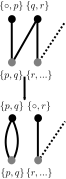
\includegraphics[width=.13\textwidth]{figures/scaj_algorithm_cases_i.pdf}}\quad
\subfigure[]{\includegraphics[width=.115\textwidth]{figures/scaj_algorithm_cases_ii.pdf}}\quad
\subfigure[]{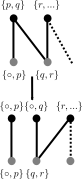
\includegraphics[width=.16\textwidth]{figures/scaj_algorithm_cases_iii.pdf}}\quad
\subfigure[]{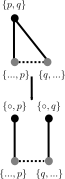
\includegraphics[width=.13\textwidth]{figures/scaj_algorithm_cases_iv.pdf}}

%	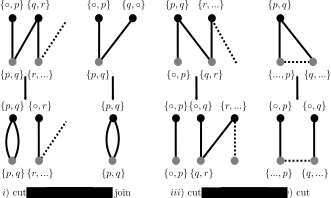
\includegraphics[width=0.6\textwidth]{figures/scaj_algorithm_cases.pdf}
	\caption{Cases $a)-d)$ of the algorithm for sorting $\alpha$ into 
		$\alpha'$ under $\m{SCAJ}$ shown on the adjacency graph. Top) components of
		$AG(\alpha,\alpha')$ and bottom) resulting components of $AG(\alpha \circ \rho,\alpha')$, where $\rho$ is
	either a cut, a join, or a cut-and-join with $(\alpha,\alpha\circ\rho)\in \m{SCAJ}$ and 
	$d_{\m{SCAJ}}(\alpha,\alpha')>d_{\m{SCAJ}}(\alpha\circ\rho,\alpha')$.}
	\label{fig:scaj_algorithm_cases}
\end{figure}

\paragraph{Open Problems}

The complexity of other rearrangement problems and the distance problem where only linear chromosomes are allowed remain open.

\subsection{Double-Cut and Join Model}
\label{sec:dcj}

The $\m{DCJ}$ model acts on mixed genomes.
This is the case, e.g., for genomes that contain plasmids in addition to the linear
chromosomes~\cite{Casjens_2000,Qiu_2004,Volff_2000} or in tumor genomes~\cite{Raphael_2004}.
In the $\m{DCJ}$ model an event cuts two adjacencies and forms two new 
adjacencies by joining four telomeres, see \Cref{fig:DCJ_events}. 
More formally, a pair of genomes $(\alpha,\alpha')$ is
an event in $\m{DCJ}$ if and only if $(\alpha,\alpha')\in \m{SCAJ}$ or there
exist $p, q, r, s\in \mathcal{E}(\alpha)$ such that
$\alpha\cup\{\{p,s\},\{r,q\}\}=\alpha'\cup\{\{p,q\},\{r,s\}\}$ (double-cut and
join).
%
Translocations, fusions, fissions, and inversions are represented directly in $\m{DCJ}$. 
The operations block-interchange and transposition are included indirectly via two $\m{DCJ}$ operations: 
the excision of a circular intermediate and the reinsertion at a different position. 
This can be implemented naturally by assigning a weight of two to
block-interchanges and transpositions and a weight of one to translocations,
fusions, fissions, and inversions~\cite{Yancopoulos_2005}.
The occurrence of such implicit transpositions, i.e., two consecutive $\m{DCJ}$ rearrangements that are equivalent to a transposition, 
in parsimonious $\m{DCJ}$ scenarios was estimated to $17\%$ of the rearrangement mutations for mammalian genomes~\cite{Jiang_2015}. 

\begin{figure}
	\begin{center}
		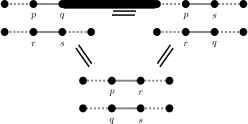
\includegraphics[width=0.42\textwidth]{figures/dcj_genome_graph.pdf}
	\end{center}
	\caption{Application of double-cut and join operation to adjacencies visualized on the genome graph.
		Note that the events of the submodel $\mathcal{SCAJ}$
		which are illustrated in \Cref{fig:SCAOJ_events} are also events of
		$\mathcal{DCJ}$. }
	\label{fig:DCJ_events}
\end{figure}

\paragraph{Polynomial Time Solvable Problems}

The distance problem under $\m{DCJ}$ can be computed in linear time 
using the breakpoint graph~\cite{Yancopoulos_2005}.
The $\m{DCJ}$ distance for two genomes $\alpha$, $\alpha'$ can be computed by
$d_{\m{DCJ}}(\alpha,\alpha')=b-c$, 
where $b$ is the number of breakpoints and $c$ is the
number of cycles in $BP(\alpha,\alpha')$. 
The web service \texttt{CEGeD} can be used to solve the distance problem
under $\m{DCJ}$, see \Cref{table:tools}.
In order to apply the breakpoint graph
for multichromosomal genomes so called capping, i.e., 
the addition of auxiliary end elements, and the concatenation of linear chromosomes is needed~\cite{Yancopoulos_2005}.

By using the adjacency graph a linear time algorithm was presented which has
the advantage that also multichromosomal genomes are covered naturally~\cite{Bergeron_2006}.
With respect to the adjacency graph the $\m{DCJ}$ distance is computed as 
$d_{\m{DCJ}}(\alpha,\alpha')=N-(C+I/2)$ 
for two genomes $\alpha,\alpha'$ with $N$ genes where $C$ is the
number of cycles and $I$ is the number of odd paths in $AG(\alpha,\alpha')$.
%
The equivalence of the two distance formulas follows from the following facts: 
\begin{inparaenum}[i)]
	\item the number of breakpoints $b$ equals
	$N+t_{\alpha}/2+E_{\alpha'} =
	N+t_{\alpha'}/2+E_{\alpha}$, where
	$t_{\beta}$ is the number
	of telomeres of a genome $\beta$ and $E_{\beta}$ is the number of
	$\beta$-paths,
	\item $t_{\alpha}/2+t_{\alpha'}/2 = I+E$ and
	$E=E_{\alpha}+E_{\alpha'}$, and
	\item $c=C+I+E$.
\end{inparaenum}

In the following a sketch of the proof of correctness of the 
$\m{DCJ}$ distance formulas is given, for details see~\cite{Bergeron_2006}. An alternative 
derivation is presented in~\cite{Bergeron_2013}. 
The adjacency graph of two equal genomes consists of one-cycles ($C_2$) - one
such cycle for each adjacency - and odd paths of length one ($I_1$) - one such path for each telomere. 
Hence sorting is equivalent to choosing $\m{DCJ}$ 
events which increase the number of $C_2$ or $I_1$. Since a $\m{DCJ}$ operation can:
\begin{inparaenum}[i)]
	\item not modify the number of cycles and odd paths simultaneously,
	\item increase the number of cycles at most by one, and
	\item increase the number of odd paths at most by two 
\end{inparaenum}
it follows that $d_{\m{DCJ}}(\alpha,\alpha')\geq N-(C+I/2)$ holds. 
% 
The tightness of this bound was shown by giving a greedy algorithm that 
always attains the bound. In each step the greedy algorithm can apply one of the following 
two cases, see \Cref{fig:dcj_algorithm_cases}. Case 1: In
the presence of the adjacencies $\{p,q\}\in \alpha'$ and $\{o,p\}, \{q,r\}\in \alpha$ the $\m{DCJ}$ event is 
$(\alpha,\{\alpha \setminus	\{\{o,p\},\{q,r\}\}\} \cup \{\{p,q\}, \{o,r\}\})$.
This creates a new one-cycle and reduces the size of a path by
two.
Case 2: For telomeres $\{p,\circ\}, \{q,\circ\}\in \alpha'$ and an adjacency
$\{p,q\} \in \alpha$ the $\m{DCJ}$ event is $(\alpha,\{\alpha \setminus
\{p,q\}\} \cup \{\{p,\circ\},\{q,\circ\}\})$. This replaces an even path of
length two by two odd paths of length one. Observe that the second event uses only one cut.

In~\cite{Bergeron_2006} a linearization of a circular genome is modeled by an additional cut of a vestigial adjacency 
$\{\circ,\circ\}$ and two joins of the resulting telomeres to telomere adjacencies, see~\cite{Friedberg_2008} for a 
detailed description.


\begin{figure}
% 	\begin{center}
% 		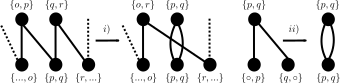
\includegraphics[width=0.8\textwidth]{figures/dcj_algorithm_cases.pdf}
% 	\end{center}
	\centering
	\subfigure[Case 
	1]{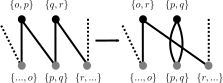
\includegraphics[width=.45\textwidth]{figures/dcj_algorithm_case_1.pdf}}\quad 
	\subfigure[Case 2]{
	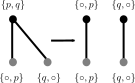
\includegraphics[width=.27\textwidth]{figures/dcj_algorithm_case_2.pdf}}
	\caption{The two cases of the $\m{DCJ}$ sorting algorithm~\cite{Bergeron_2006} shown for the adjacency graph.}
	\label{fig:dcj_algorithm_cases}
\end{figure}
%
%-DCJ operation applied to two adjacencies of same genome disconnects the
%incident edges of AG, and reconnects them in one of the possible other ways
%
%-dcj sorting operation acts on single path or cycle or on two even paths of the
%adjacency graph

\paragraph{NP-Hard Problems}

% distance unsigned %
Many experimental studies do not determine the strandedness of the genes~\cite{Chen_2010}. 
In such cases genomes are commonly represented by
\emph{unsigned permutations}. This motivates the \emph{sorting problem for unsigned genomes (SUG)} under 
$\m{DCJ}$ which was studied for the first time in~\cite{Chen_2010}. The NP-hardness of this problem for 
unichromosomal unsigned genomes was shown by a reduction from the NP-hard 
\emph{breakpoint graph decomposition (BGD)} problem~\cite{Kececioglu_1995}. 
The BGD problem is to find a decomposition of a breakpoint graph into a maximum number of edge-disjoint 
alternating cycles. Note that in contrast to the case of signed genomes in the breakpoint graph for unsigned 
genomes each gene corresponds to a single vertex. 
An approximation algorithm for solving the SUG problem for multichromosomal
mixed genomes was presented in~\cite{Chen_2010}. The algorithm is based on a modification of the approximation algorithm of~\cite{Lin_2008} 
for the BGD problem. 
%An improved approximation algorithm has been given in~\cite{Chen_2011}. 

Recall that similar to $\m{DCJ}$ also for $\m{INV}$ the distance problem for signed genomes is 
polynomial time solvable~\cite{Hannenhalli_1999} whereas it is NP-hard for unsigned genomes~\cite{Caprara_1997}. 
This suggests that the complexity of the distance problem for rearrangements that cut and join two adjacencies is 
rather dependent on the availability of gene strandedness information than on the set of allowed rearrangement events.

% median problem, double distance, guided halving %
The median problem under $\m{DCJ}$ was shown to be NP-hard by reduction of 
the BGD problem~\cite{Tannier_2009}. Note that also this result holds analogously for the $\m{INV}$ model~\cite{Caprara_2003}. 
Since the median problem is NP-hard the small and the large parsimony problem are NP-hard too. 
For the median problem exact algorithms~\cite{Xu_2008,Zhang_2009} and also heuristics~\cite{Adam_2008,Lenne_2008} have been 
presented in the literature. 
Based on the heuristic median solver an algorithm for the small phylogeny problem has been developed in~\cite{Adam_2008}.
Examples of software tools which can be used to solve the small parsimony
problem under $\m{DCJ}$ are \texttt{MGRA} and \texttt{PATHGROUPS}, see
\Cref{table:tools}.

\paragraph{Applications}
In \cite{Bergeron_2010} the distance problems under $\m{SCAJ}$ and
$\m{DCJ}$ have been calculated for $281$ synteny blocks of the human-mouse
comparison from \cite{Pevzner_2003} and for $1359$ synteny blocks of the genomes
of chimp, rhesus monkey, mouse, rat, and dog from \cite{Ma_2006} with respect to
the human genome. 
The results show that the obtained distances under $\m{SCAJ}$ are much
larger than the distances under $\m{DCJ}$. The authors stress that the goal of  
the $\m{SCAJ}$ model is rather an indicator for evaluating results under 
the $\m{DCJ}$ model than being a realistic evolutionary model. 
Based on their results, the authors suggest that
single-cut operations are more important in the mouse-human evolution than in 
the chimp-human evolution.
The pairwise $\m{DCJ}$ distance between synteny blocks from genomes of
\emph{Shigella boydii}, \emph{Shigella dysenteriae}, \emph{Shigella flexneri}, 
and \emph{Escherichia coli} have been calculated in \cite{Friedberg_2008}. The generation of the synteny blocks and the calculation
of the $\m{DCJ}$ distances have been made by \texttt{Mauve}, see
\Cref{table:tools} for more information.
 
The algorithm for the small phylogeny problem which has been developed
in~\cite{Adam_2008} was used to analyze $13$ chloroplast DNAs of genomes of 
\emph{Campanulaceae} and the mammalian dataset from \cite{Murphy_2005}
(including the presented phylogenetic tree)  which consists of the genomes of
human, rat, mouse, cat, dog, pig, and cow.
The results show that the reconstructed ancestral genomes contain between $1$
and $5$ circular chromosomes that occur in immediate ancestors of the seven
mammalian species. The total number of used $\m{DCJ}$ operations is $486$ and 
the total number of restricted $\m{DCJ}$ operations, i.e., $\m{DCJ}$
operations that do not produce any circular chromosomes, is $487$.
This result strengthens the conjecture that there is no biological evidence of circular chromosomes in the
nuclear genomes of higher eukaryotes \cite{Brown_2006}.

Many software tools are based on the $\m{DCJ}$ model, see \Cref{table:tools} for a overview.
For instance, \texttt{GEvolutionS} can be used to simulate evolutionary
genome rearrangement scenarios and  \texttt{MLGO} and \texttt{GREDU} can be
used for the case that the input genomes do not have the same gene content.

\subsection{Multi-Cut and Join Model}

%motivation
Rearrangement operations like inversions, fusions, fissions, and translocations
can easily be modeled by cutting a genome at two positions before applying rejoin operations. However, rearrangement 
operations that create three breakpoints, e.g., transpositions and inverse
transpositions, i.e., transpositions were in addition the orientation of the
transposed genes is changed, can be modeled only indirectly when at most two cuts are allowed, e.g., 
by using a pair of $\m{DCJ}$ operations or three $\m{SCAJ}$ operations.
%
Therefore, a generalized rearrangement model has been suggested~\cite{Alekseyev_2008} which cuts a genome at 
$k\in \mathbb{N}$ positions followed by rejoining the resulting fragments into new order.
The resulting model is called \emph{multi-cut and join} model ($\m{MCJ}$) 
and for a specific $k\in \mathbb{N}$ we refer it as 
\emph{$k$-cut and join} model ($\m{KCJ}$)
\footnote{
In~\cite{Alekseyev_2008} these rearrangements are called \emph{multi-break} 
rearrangements.}.
Formally, a pair of genomes $(\alpha,\alpha')$ is an event in $\m{KCJ}$ if and
only if $(\alpha,\alpha')\in (\m{K}-1)\m{CJ}$ or there exists a set of $k$
adjacencies $K \subset \alpha$ such that $\alpha' \cup
K = \alpha \cup X$, where $X$ is a subset of $\{\{x,y\}:x,y\in
\m{E}(K), x\neq y\}\cup \{\{p,\circ \}:p\in \m{E}(K)\}$ such that
$\m{E}(X)\cup \{p:\{p,\circ \}\in \mathcal{T}(X)\}=\m{E}(K)\cup \{p:\{p,\circ \}\in \mathcal{T}(K)\}$, $|X|=k$, $X\cap K = \emptyset$,
$1\m{CJ}=\m{SCAJ}$, and $2\m{CJ}=\m{DCJ}$.
Note that for all $i\in [1:k-1]$ this definition implies that a
$(\m{K}-i)\m{CJ}$ event is a particular event of $\m{KCJ}$ which can be
understood as a $k$-cut and join event which leaves exactly $i$ of the $k$ adjacencies unchanged.

\paragraph{Polynomial Time Solvable Problems}

The distance problem under $\m{KCJ}$ can be solved in polynomial time 
by computing
$d_{\m{KCJ}}(\alpha,\alpha')=\lceil(N-C_s(\alpha,\alpha'))/(k-1)\rceil$ for
genomes $\alpha$ and $\alpha'$, where $k\geq 2$ is the number of cuts and
$C_s(\alpha,\alpha')$ is the size of the maximum partition of the cycles in
$BP(\alpha,\alpha')$ where the total number of black edges in each subset of
cycles is equal to $1 \bmod{(k-1)}$~\cite{Alekseyev_2008}.
For instance, $C_2(\alpha,\alpha')$ equals the number of cycles in $BP(\alpha,\alpha')$ (since
for any number $c$ of cycles $(c\equiv 1)\bmod{1}$) and $C_3(\alpha,\alpha')$
gives the number of odd cycles in $BP(\alpha,\alpha')$.
Hence for $k=2$, the formula equals the $\m{DCJ}$ distance formula presented in~\cite{Yancopoulos_2005}. 
Further, two algorithms for computing the distance formula between two genomes -- a dynamic programming algorithm 
which is practical for small values of
$k$ and a linear time algorithm with exponential (in
$k$) time preliminary computations -- were presented in~\cite{Alekseyev_2008}.


\paragraph{Open Problems}
The distance problem under $\m{KCJ}$ for linear multichromosomal
genomes was studied in~\cite{Alekseyev_2008b} resulting in lower bounds for the
rearrangement distance. To the best of our knowledge no additional polynomial time algorithms have been published for 
the median problem and the small/large parsimony problem.


\section{Rearrangement Models with Intergenic Regions}

% When intergenic regions are considered the weight of an edge equals to the size
% of the intergenic region between genes $x$ and $y$. The weight of a genome $w(\alpha)$
% is then the total size if the intergenic regions of $\alpha$.

This section reviews results that incorporate the sizes of intergenic regions
into the models for rearrangement analysis. In recent years researchers have
argued that the sizes of intergenic regions can be relevant information for
rearrangement analysis in order to improve phylogenetic distance estimation.

To incorporate the sizes of the intergenic regions into the rearrangement models,
weighted genome graphs can be defined where each edge $\{p,q\}$ has a weight if
$p$, $q$ are extremities of neighboring genes or $q=\circ$ and $\{p,\circ\}$ is a
telomere. The weight of an edge equals the size of the corresponding intergenic
region, i.e., the intergenic region between the two neighboring genes,
respectively the size of the intergenic region between the gene and the
telomere. The weight $w(\alpha)$ of a genome $\alpha$ is then the sum of the
weights of all edges of the genome graph of $\alpha$, i.e., the total size of all
intergenic regions of $\alpha$. Then, weighted versions of the genome
rearrangement problems can be defined. A weighted single-cut or join model is a
single-cut or join model where the weight of the adjacency that is broken by a
cut equals the sum of the weights of the two telomeres that are created and the
sum of the weights of the adjacency that is formed by a join equals the sum of
the weights of the two telomeres that are connected. Weighted versions of
single-cut and join models or multi-cut and join models are defined analogously.

The computational complexity and approximation-algorithms are known for various
weighted rearrangement problems that consider the size of intergenic regions.
Sorting with weighted reversals for unsigned permutations~\cite{brito2020sorting} and for signed
permutations \cite{oliveira2020sorting} is NP-hard. The former problem has a 4-approximation algorithm
\cite{brito2020sorting} and the latter problem has a 2-approximation algorithm \cite{oliveira2020sorting}. Sorting with
weighted reversals and weighted transpositions problem is NP-hard for unsigned
and signed permutations \cite{oliveira2021sorting}. The former problem has a 4-approximation algorithm
\cite{dias2019block} and the latter problem has a 3-approximation algorithm \cite{oliveira2021sorting}. Sorting with
weighted transpositions for unsigned permutations is NP-hard \cite{oliveira20203} (Note, that
already the unweighted version of this problem is NP-hard~\cite{Bulteau_2012}) and has
3.5-approximation algorithms~\cite{oliveira20203}. The Block-Interchange is a rearrangement event
that swaps the position of two segments (not necessarily consecutive) of the
genome. The sorting by intergenic block-interchange problem has a
2-approximation algorithm \cite{dias2019block} and its complexity is unknown.

A weighted version of the DCJ distance problem was studied in~\cite{fertin2017algorithms} where a
weighted DCJ operation was defined as a DCJ operation which changes the weights
of the edges such that the sum of the weights of the two cutted edges equals the
weights of the two joined edges and the weights of all other edges do not
change.  It was shown that the wDCJ distance problem is strongly NP-hard and has
a $4/3$-approximation algorithm.

There exist mutations that change the size of intergenic regions but do not
change the order of the genes. To consider such mutations within the
rearrangement models an $i$-indel operation is defined as an operation that
changes the size of an intergenic region. The weight of an i-indel operation is
the corresponding amount of size change. The sorting problem for the wDCJ model
with i-indel operations (i.e., to find a shortest wDCJ scenario with minimum
total weight of the i-indel operations) can be solved in time $O(n\log n)$ \cite{bulteau2016genome}.
Several approximation algorithms have been designed for the problem of sorting
unsigned permutations with $i$-indels in \cite{alexandrino2021incorporating}: i) 4-approximation algorithm for
sorting with $i$-indels and weighted reversals has a, ii) a 4.5-approximation
algorithm for sorting with $i$-indels and weighted transpositions, and iii) a
6-approximation algorithm for sorting with $i$-indels, weighted reversals, and
weighted transpositions. For signed permutations the latter problem has a
3-approximation algorithm \cite{alexandrino2021reversal}.

Since also the gene order rearrangement operations might change the size of the
intergenic regions corresponding extended gene order rearrangement operation
have been studied. Transpositions that might remove a part of an intergenic
region (i.e., a part of the genome that does not contain a gene) to include it
into another intergenic region has been considered in \cite{oliveira2021sorting,dias2019block}. It was shown that
for such generalized transpositions improved approximation algorithms exist for
the following cases: i) a 2.5-approximation algorithm for sorting unsigned
permutation with (generalized) weighted transpositions~\cite{oliveira2021sorting} and ii) sorting with
(generalized) weighted transpositions for signed permutations and unsigned
permutations has a 2.5-approximation algorithm \cite{oliveira2021sorting}, respectively 3-approximation
algorithm \cite{dias2019block}.

\section{Preserving Genome Rearrangement Models}
\label{sec:preserving_models}


This section discusses the sorting problem, the median problem, and the small parsimony problem under $\m{INV}^{p}$. 
Some results for related preserving rearrangement models are discussed at the end of the section.

% preserving inversion intro
The sorting problem under $\m{INV}^{p}$ has been introduced in~\cite{Figeac_2004} with the objective to 
produce biologically more relevant results.
%
Unfortunately, the sorting problem under $\m{INV}^{p}$ is NP-hard~\cite{Figeac_2004}. But, it is 
fixed-parameter tractable~\cite{Bouvel_2011} 
and there exist linear run time algorithms for many relevant instances~\cite{Berard_2007,Berard_2008b}, and 
algorithms with a polynomial average run time~\cite{Bouvel_2011}.
% 
Algorithms for the median problem and the small parsimony problem under $\m{INV}^{p}$ that have a polynomial run time 
for many relevant data sets have been proposed in~\cite{Bernt_2012,Bernt_2008}, see \Cref{sec:rev_p_sorting}.



%SIT
\subsection{Strong Interval Tree}
\label{sec:SIT}

The strong interval tree (SIT)\footnote{Note that strong interval trees are similar to PQ-trees~\cite{Booth_1976}.} is the 
central data structure for efficient preserving rearrangement analysis. The main reason is that the SIT can be computed in linear 
time and represents the common intervals (which can be quadratic in
number) in linear space~\cite{Berard_2007}.

Let $\Pi$ be a set of $k$ genomes that are represented by signed permutations and $\lambda$ be a consistent reference permutation (typically $\lambda\in\Pi$). 
A common interval $I \in C(\Pi)$ is \emph{strong} if every other common
interval in $C(\Pi)$ is either included in $I$ or it includes $I$. By
definition the strong intervals of $\Pi$ form a hierarchy which is captured by the
\emph{strong interval tree} (SIT). The SIT of $\Pi$ with respect to $\lambda$, denoted by ${T}^{\lambda}(\Pi)$, is an ordered tree where each vertex represents a strong common interval of $\Pi$ and the edges represent the minimum inclusion relation. The order of the children of a vertex in the SIT are without loss of generality given by their order in the reference permutation $\lambda$.
For every inner vertex $I$ of a SIT with children $I_1,\ldots,I_l$ that are ordered according to the reference permutation $\lambda$ the \emph{quotient permutation} associated with $I$ for $\pi\in \Pi$ is the permutation
$\pi_I^\lambda$ which satisfies that $\pi^\lambda_I(i)$ precedes
$\pi^\lambda_I(j)$ if and only if $I_i$ is to left of $I_j$ in $\pi$, for $i\neq j$.
A quotient permutation is called \emph{linear increasing} if it is equal to
$\iota$, \emph{linear decreasing} if it is $(l\ (l-1)\ldots 1)$, and \emph{prime} otherwise. 
A vertex $I$ of a SIT is called \emph{linear} if all $k$ quotient
permutations are either linear increasing or linear decreasing. Otherwise it is called \emph{prime}. It holds that a vertex
of a SIT is linear if and only if every union of consecutive children is a
common interval, whereas for a prime vertex only the union of all children
is a common interval~\cite{Berard_2007}.

A so called \emph{$k$-sign} $\{+1,-1\}^k$ is assigned to the vertices to represent
the orientation of linear quotient permutations and the orientation of the elements in the case of leaf vertices. 
%
For a vertex $I$ the $i$-th element of a $k$-sign, denoted by $s(i)$, is
determined based on the following rules:
\begin{inparaenum}[i)]
\item A leaf $I$ has $s(i)=+1$ if the corresponding element has the same sign
	in $\pi_i$ as in $\lambda$ and $s(i)=-1$ otherwise. 
\item A linear inner vertex $I$ has $s(i)=+1$ if $\pi_{iI}^\lambda$ is the
	identity permutation and $-1$ otherwise.
\item A prime vertex with linear parent inherits the $k-sign$ of the parent. 
\end{inparaenum}
A SIT is \emph{unambiguous} if every prime vertex has a linear parent and
\emph{ambiguous} otherwise.
SITs without prime vertices are called \emph{definite}.
In the \emph{signed quotient permutation} each element is assigned the sign of the 
corresponding child node, i.e., $\pi_{iI}^\lambda(j)$ is assigned the $i$-th 
component of the $k$-sign of the $j$-th child. 
For a linear vertex $I$ of the SIT a sign $s_I(i)$ contains the same
information as the quotient permutation $\pi_{iI}^\lambda$, i.e., there is a
bijective relation between signs of linear vertices of definite SITs and
consistent permutations.
% Note that a set of genes is a common interval of $\Pi$ if it is
% Note that a set of genes is a common interval of $\Pi$ if it is
% either a vertex of $\MB{\m{T}}{T}_\lambda(\Pi)$ or the union of consecutive children of a
% linear vertex of $\MB{\m{T}}{T}_\lambda(\Pi)$~\cite{Berard_2007,Bernt_2009}.
Note that these rules uniquely determine the signs of every vertex of
unambiguous and definite SITs, but 
the signs of a prime root vertex and prime vertices with prime parent in 
ambiguous trees are not determined.
An example illustrating a SIT for a set of permutations is shown in
\Cref{fig:SIT_def_definit}.

\begin{figure}
		\begin{center}
			\subfigure[]{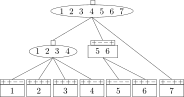
\includegraphics[width=0.45\textwidth]{figures/SIT_definition.pdf}}\label{subfi:SIT_def_definit_a}\quad
			\subfigure[]{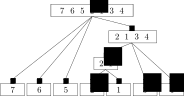
\includegraphics[width=0.45\textwidth]{figures/SIT_linear_corrected.pdf}\label{subfi:SIT_def_definit_b}}
		\end{center}
	\caption{(a) Strong common interval tree of $\Pi=\{(1 \ldots 7),$ 
	$(-{7}~1~3~2~4~6~-{5}),$ $(6~-{5}~-{4}~3~-{1}~2~7),$
	$(-{5}~-{6}~7~3~4~2~-{1})\}$ where the trivial common
	intervals, $\{5,6\}$, and $\{1,2,3,4\}$ are
	the strong common intervals of $\Pi$. Prime vertices and linear vertices are represented 
	by ellipses and rectangles, respectively. The root vertex and vertex $\{1,2,3,4\}$ are prime and vertex $\{5,6\}$ is 
	linear increasing with respect to $(1 \ldots 7)$.
	%
	(b) Definite SIT ${T}^\iota(\Sigma)$ for
	$\Sigma=\{(7~6~5~-{2}~1~-{3}~-{4}), \iota\}$. Note that every vertex is
	linear since every union of consecutive children of each vertex is a common
	interval of $\Sigma$. The signs of the vertices are shown at the top of the
	rectangles. The signs with respect to $\iota$ are omitted since it is $+$
	for all vertices. Vertex $\{2,1\}$ is linear decreasing since its quotient
	permutation is $(2~1)$ and the quotient permutation $(1~2~3)$ of vertex
	$\{2,1,3,4\}$ implies that it is linear increasing. A scenario sorting
	$\pi_1=(7~6~5~-{2}~1~-{3}~-{4})$ to
	$(-{7}~-{6}~-{5}~-{4}~-{3}~-{2}~-{1})$ is obtained by
	applying inversions $\{7\}$, $\{6\}$, $\{5\}$, $\{4\}$, $\{3\}$, $\{1\}$,
	$\{1,2\}$, and $\{1,2,3,4\}$ to $\pi_1$.
	Recall that $\iota$ and $(-{7}~-{6}~-{5}~-{4}~-{3}~-{2}~-{1})$ are
	considered to be equal.}
	\label{fig:SIT_def_definit}
\end{figure}




\subsection{Algorithms for the Preserving Inversion Model}
\label{sec:rev_p_sorting}

Algorithms for the sorting problem under $\m{INV}^p$ for signed unichromosomal
linear genomes and a partition of the set of problem instances
into instances, that can be solved in linear time, polynomial time, or
exponential time have been presented in~\cite{Berard_2007}. More precisely, problem instances with a definite SIT can be solved in linear time, those with an unambiguous SIT can be solved in sub-quadratic time, and instances with an ambiguous SIT have a worst case exponential run time.

\begin{figure}
	\begin{center}
		\subfigure[]{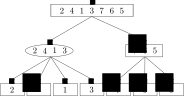
\includegraphics[width=0.45\textwidth]{figures/SIT_unambiguous.pdf}\label{subfi:SIT_un_ambiguous_a}}\quad
		\subfigure[]{\includegraphics[width=0.45\textwidth]{figures/SIT_ambiguous.pdf}\label{subfi:SIT_un_ambiguous_b}}
	\end{center}
% 		\begin{center}
% 			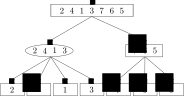
\includegraphics[width=0.4\textwidth]{figures/SIT_unambiguous.pdf}\quad
% 			\includegraphics[width=0.4\textwidth]{figures/SIT_ambiguous.pdf}
% 		\end{center}
	\caption{(a): Unambiguous SIT ${T}^\iota(\Pi)$ for
	$\Pi=\{\pi=(2~-{4}~1~3~-{7}~-{6}~-{5}),\iota\}$.
	Vertex $\{2~4~1~3\}$ is prime since its quotient
	permutation is $(2~4~1~3)$.
	Its parent vertex is linear increasing which results in an unambiguous SIT. A parsimonious scenario
	sorting $(2~-{4}~1~3)$ to $\iota$ is given by the inversions
	$\{1,3,4\}$, $\{2,3\}$, $\{3\}$, and $\{1,2,3\}$.
	Applying the scenario to $\pi$ yields
	$\pi'=(1~2~3~4~-{7}~-{6}~-{5})$
	which has a definite SIT ${T}^\iota(\pi',\iota)$. For $\pi'$ the 
	inversion $\{5,6,7\}$ is a parsimonious
	scenario.
	Both scenarios together are a parsimonious scenario for the unambiguous SIT ${T}^\iota(\Pi)$.
	%
	(b): Example of an ambiguous SIT. Here, the signs of
	prime vertices of ${T}^\iota(\{(3~1~-{5}~7~-{4}~6~-{2}),\iota\})$ are not
	uniquely determined.
% 	A parsimonious scenario is obtained by applying the algorithm for
% 	unambiguous SITs for every sign combination which results to an exponential
% 	run time in worst case. 
	A parsimonious scenario is obtained by a negative sign
	for the root vertex and a positive sign for its child prime vertex.}
	\label{fig:SIT_un_ambiguous}
\end{figure}


In the following we will identify inversions by the interval that they reverse. 
Consider a signed permutation $\pi$ that is to be transformed into $\iota$. 
Note that arbitrary pairs of signed permutations can be reduced to this case 
by renaming the elements of the permutations. 
Let ${T}^\iota(\Pi)$ be the strong interval tree of $\Pi=\{\pi,\iota\}$.
Instead of the $2$-sign at each prime vertex with linear parent and each linear
vertex a $1$-sign (or just sign for short) is stored at the vertices. The 
sign is equal to the $2$-sign component that corresponds to $\pi$. 
This is because the sign of the target permutation $\iota$ is $+$ for all vertices 
with a sign. 
Therefore, we can call a vertex linear increasing (resp. decreasing) if 
the quotient permutation is linear increasing (resp. decreasing). 
% The vertices of $\MB{\m{T}}{T}_\iota(\Pi)$ get assigned signs $+$ or $-$ according
% to the following rules 
% \begin{inparaenum}[i)]
% 	\item leafs get the sign of the corresponding element,
% 	\item linear increasing vertices get a ``+'',
% 	\item linear decreasing vertices get a ``-'', and 
% 	\item prime vertices with linear parent get the sign of the parent.
% \end{inparaenum}

The key for solving the sorting problem under $\m{INV}^p$ is that 
an inversion is preserving if and only if it is a vertex of the SIT or a union 
of children of a prime vertex \cite{Berard_2007}. Thus, linear vertices can 
only be reversed as a whole whereas the children of prime vertices can be freely rearranged. With respect to the SIT the problem of sorting by preserving inversions 
is to apply rearrangements such that all quotient permutations are transformed 
into the identity permutation, i.e., the vertices become linear increasing. 
Hence, if a the sign of vertex $I$ of ${T}^\iota(\pi)$ is different to the sign of its
parent vertex, it holds that the inversion defined by $I$ is always part of any
optimal sorting scenario~\cite{Berard_2007} (Lemma 2), i.e., 
the inversions that correspond to vertices with a sign different to the one of their parent define a parsimonious scenario~\cite{Berard_2007} (Theorem 2).
This can easily be implemented to run in linear time, see \Cref{subfi:SIT_def_definit_b} for an example. 
Since the inversions in parsimonious preserving scenarios for a problem instance with a definite strong interval tree commute the set of all parsimonious scenarios can be obtained easily.

For a problem instance with unambiguous SIT a method to transform the signed quotient
permutation of prime vertices into the identity permutation is needed. 
Since the children of a prime vertex can be freely rearranged a solution is 
to reconstruct an unconstrained parsimonious inversion scenario for the signed quotient 
permutation. That is, for every prime vertex $I$ a parsimonious scenario from $\pi^\lambda_I$ to $\iota$ is computed 
if $I$ has a positive sign. If it has a
negative sign a scenario from $\pi^\lambda_{I}$ to $(-{n}~\ldots~-{1})$ is
computed.
Applying the corresponding inversions to $\pi$ results in a definite SIT which can be processed as explained beforehand.
%
The run time of the algorithm for unambiguous SITs is dominated by solving the sorting problem for prime vertices
which is done by the algorithm presented in~\cite{Tannier_2007}.
The algorithm from~\cite{Tannier_2007} solves the sorting problem under
$\m{INV}$ for signed permutations in  sub-quadratic run time
$O(n\sqrt{n\log{(n)}})$. An example for sorting an
unambiguous SIT under $\m{INV}^p$ is given in \Cref{subfi:SIT_un_ambiguous_a}.

For ambiguous SITs the signs of prime vertices with prime parent are unknown,
see \Cref{subfi:SIT_un_ambiguous_b}. 
By trying every combination of sign assignments and applying the algorithm for unambiguous SITs an exact solution can be obtained. 
An improvement is possible by applying dynamic programming separately for every component of connected 
prime vertices. 
Assume that $u\in\mathbb{N}$ unsigned prime vertices exist, in this
case the described algorithm for ambiguous SITs (which uses the algorithm
from~\cite{Tannier_2007}) has an exponential run time of
$O(2^{u}n\sqrt{n\log{(n)}})$ in the worst case.


% solving small parsimony problem 
% \subsection{Preserving Inversion Phylogeny Reconstruction}
% \label{sec:rev_p_parsimony}

In the following the algorithm of~\cite{Bernt_2012} for the small parsimony
problem under $\m{INV}^p$ for sets of genomes with a definite SIT is presented.
The algorithm runs in polynomial time. 
The basis of the approach is an extension of the results of~\cite{Berard_2009}
which was first used in an approach for solving the preserving inversion median problem~\cite{Bernt_2008}. 
The idea of the algorithm is to extract binary characters from the SIT which are then processed by Fitch's algorithm~\cite{Fitch_1971} for
maximum parsimony. \Cref{fig:SIT_parsimony} 
illustrates the algorithm which is described below.


\begin{figure}
	\begin{center}
		\subfigure[]{\includegraphics[width=0.46\textwidth]{figures/SIT_parsimony_1.pdf}\label{subfig:SIT_parsimony_a}}\quad
		\subfigure[]{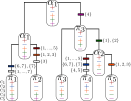
\includegraphics[width=0.44\textwidth]{figures/SIT_parsimony_2.pdf}\label{subfig:SIT_parsimony_b}}
	\end{center}
% 	\begin{center}
% 		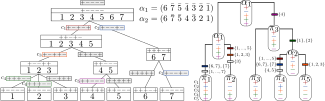
\includegraphics[width=\textwidth]{figures/SIT_parsimony.pdf}
% 	\end{center}
	\caption{(a): SIT ${T}^\iota(\Pi)$ with $k$-signs for $\pi_1=\iota$,
	$\pi_2=(6~-{7}~3~-{2}~-{1}~4~5)$,
	$\pi_3=(6~-{7}~-{5}~4~-{3}~-{2}~-{1})$,
	$\pi_4=(-{7}~-{6}~-{1}~-{2}~3~-{5}~4)$, and
	$\pi_5=(6~-{7}~-{5}~4~-{1}~-{2}~3)$.
	%
  %A $k$-sign is shown as strings on $\{+,-\}$ on top of each vertex.
	%
  %The $k$-sign of vertex $\{3\}$ is $(++-++)$ since element $3$ has a
  %positive
	%sign in $\pi_1,\pi_2,\pi_4$, and $\pi_5$ and a negative sign in $\pi_3$.
	%
% 	For vertex $\{4,5\}$ the $k$-sign is $(++---)$ since element $4$ proceeds element
% 	$5$ in $\pi_1$ and $\pi_2$ and $4$ succeeds $5$ in $\pi_3,\pi_4$, and $\pi_5$.
	%
	The character state of a vertex is placed on the edge to its parent.
	%
	Character state assignments of vertex $\{1\}$	is $(+++--)$ because the $k$-signs of vertex $\{1\}$ and vertex
	$\{1,2,3\}$ are equal in the first three positions and unequal in positions
	four and five.
	%
	SIT ${T}^\iota(\Pi)$ shows five unique, nontrivial characters which are
	denoted by $c_1,\ldots,c_5$.
	%
	The permutation $\pi_2$ is uniquely determined by character states and
	$k$-signs since the signs of all vertices in pre-order are
	$-1,+1,-1,-1,-1,+1,+1,+1,+1,+1,+1,-1$.
	%
	(b): Optimal solution of the small parsimony problem under $\m{INV}^p$
	which is obtained by Fitch's algorithm~\cite{Fitch_1971} for $T$
	and nontrivial, unique characters $c_1,\ldots,c_5$.
	%
	Ancestral permutations
	$\alpha_1=(6~-{7}~-{5}~-{4}~-{3}~-{2}~-{1})$ and
	$\alpha_2=(6~-{7}~-{5}~4~-{3}~2~1)$ are determined by preserving inversions represented on the edges.
	%
	Root permutation $\alpha_1$ is constructed from $\pi_3$ by reverting element
	$\{4\}$.
	%
	This information is obtained since the character state assignment of both
	vertices differs only in one sign of $c_5$ which corresponds to vertex $\{4\}$ in the SIT.}
	\label{fig:SIT_parsimony}
\end{figure}

Again, the foundation of the algorithm is the insight that an inversion is
preserving with respect to a set of permutations $\Pi$ if and only if it is
either a vertex of ${T}(\Pi)$ or a union of consecutive child vertices of
a prime vertex. This result from~\cite{Bernt_2012} is a generalization of a result of~\cite{Berard_2007}. 
Hence, for a linear vertex preserving inversions can only change its order.
Therefore, for each linear vertex it needs to be
determined in which of the permutations it has to be inverted or not.
For a set of permutations $\Pi=\{\pi_1,\ldots,\pi_k\}$ 
the Parity Lemma~\cite{Berard_2007} and its reformulation for SITs with
$k$-signs~\cite{Bernt_2012} states that a vertex $I$ has to be inverted in
permutation $\pi_i$ in a parsimonious preserving scenario if and only if its
sign $s_I(i)$ differs from the sign $s_J(i)$ of its parent vertex $J$.
Hence, the essential information is the difference of the $k$-signs
of the vertices and their respective parents. 
To capture these differences every vertex of the SIT
${T}^\lambda(\Pi)$ is assigned to a binary character representing the
information on the equality or inequality of its $k$-signs and the $k$-signs of
its parent.
Formally, consider a non-root vertex $I$ and its parent vertex $J$ of
${T}^\lambda(\Pi)$ with $k$-signs $s_I$ and $s_J$.
The binary \emph{character state assignment} of $I$ is a 
$k$-tuple $c_I$ such that $c_I(i)=s_I(i)\cdot s_J(i)$ for $i\in[1:k]$.
The character state assignment for the root vertex is defined by comparing its
$k$-sign with $\{+1\}^k$.
Note that a character state assignment for every vertex of ${T}^\lambda(\Pi)$
uniquely determines $\Pi$ since $\pi_i$ is determined by multiplying $c_I(i)$
and parents sign $s_J(i)$ from top to bottom starting at root vertex with $+1$.
Hence, each assignment of character states to the nodes of the SIT uniquely determines a consistent permutation, see
\Cref{subfig:SIT_parsimony_a} for an example.

Due to the bijective relation between consistent permutations, character state
assignments, and preserving inversions, the small parsimony problem for a set of
permutations $\Pi$ with definite SIT and phylogenetic tree $T$ can be solved exactly and 
efficiently by solving the small parsimony problem for the character states
for the vertices of ${T}^\lambda(\Pi)$.
%
% This is done as described in the following.
%
Consider a set of permutations $\Pi$ with a definite SIT ${T}^\lambda(\Pi)$,
the character state assignments of its vertices, and a given tree $T$.
Solving the small parsimony problem for $T$ and the binary characters defined
for the vertices yields a reconstruction of ancestral character states of $T$.
%
% Note that this algorithm may result in multiple optimal solutions since
% multiple optimal solutions can be inferred for small parsimony problems on
% binary characters.
Given the ancestral character states of a vertex of $T$, the signs for the
vertices of the SIT and the corresponding permutations are constructed by the
following procedure.
%
Starting with the identity permutation all strong common intervals need to be inverted 
for which the sign differs from the one of its parent. 
%
See \Cref{subfig:SIT_parsimony_b} for an example.
% 
% In conclusion the small parsimony problem for a set of permutations $\Pi$ with
% definite SIT and a tree $T$ is solved by 
% \begin{inparaenum}[1)]
% 	\item computing $\MB{\m{T}}{T}^\lambda(\Pi)$ with $k$-signs,
% 	\item determining the character state assignments of every vertex of
% 	$\MB{\m{T}}{T}^\lambda(\Pi)$,
% 	\item solving the small parsimony problem for every character state assignment,
% 	and
% 	\item computing the ancestral gene orders from the constructed character states
% 	of inner vertices.
% \end{inparaenum}
This algorithm runs in $O(kn)$ time for a set $\Pi$ of $k$ permutations of
length $n$ if ${T}^\lambda(\Pi)$ is definite.
%
Because of the one-to-one relation between the characters defined by the SIT and 
parsimonious inversions the large parsimony problem for binary characters 
under $\m{INV}^p$ is $NP$-hard as well -- 
even for sets of permutations with definite SIT~\cite{Bernt_2012}.
%
% Interestingly, unichromosomal circular genomes are also covered by this
% approach since the circular structure is covered by SIT as well.\re{CITE??}

% \subsection{Solving the Preserving Inversion Median Problem}
% \label{sec:erv_p_median}

In~\cite{Bernt_2008} an exact algorithm -- called \texttt{TCIP} -- for the median problem under $\m{INV}^p$ was presented.
\texttt{TCIP} uses the bijective relations between consistent permutations, character state assignments, and preserving inversions 
which yields a linear run time for definite SITs.
For ambiguous SITs different unconstrained versions of the median problem 
have to be solved for the quotient permutations of prime vertices considering 
different $k$-sign assignments which significantly increases the run time of \texttt{TCIP}.
However, it has been shown empirically that median problems of random gene orders as well as organellar 
gene orders often have a definite SIT and then \texttt{TCIP} has a good performance.

\paragraph{Application}
In \cite{Bernt_2012} the small phylogeny problem has been analyzed under $\m{INV}^p$ for $4$ 
unique $\gamma$-\emph{Proteobacteria} gene orders from \cite{Belda_2005} and for a
set of \emph{Burkholderia} gene orders.
Pairwise scenarios under $\m{INV}^p$ between $16$ synteny
blocks of the X Chromosome of the human, mouse, and rat genomes from \cite{Gibbs_2004}
have been constructed in \cite{Berard_2007}. The results show that the SIT for
the rat and mouse comparison is definite and that a parsimonious preserving
scenario contains $11$ inversion. The comparison between human and rat
(resp. mouse) shows an unambiguous SIT which results into a
preserving scenario with $13$ inversions (resp. $12$ inversions).



%\subsection{Preserving Inversions, (Inverse) Transpositions and TDRLs Model}
\subsection{Related Preserving Problems}
\label{sec:CREX}

Phylogenetic reconstructions should consider all relevant rearrangement operations. 
Mitochondrial gene orders, for instance, evolve by inversions, (inverse)
transpositions, and tandem-duplication-random-loss (TDRL) events (i.e., a tandem
duplication of a continuous sequence of genes followed by the loss of one copy
of each duplicated gene~\cite{Chaudhuri_2006}).
In particular TDRLs are important rearrangement events in mitochondrial genomes~\cite{Boore_2000,Inoue_2003,San_2006}.
The algorithm \texttt{CREx} which solves the preserving sorting
problem heuristically under these four rearrangement operations has been
presented in~\cite{Bernt_2007b}.
The basic principle of \texttt{CREx} is the detection of patterns in the SIT that
determine corresponding rearrangement events: i) An inversion corresponds to a vertex with a different sign as its parent, 
ii) a transposition is represented by a vertex that has two children and its sign differs from the one of its children and its parent, 
iii) an inverse transposition corresponds to a vertex whose sign is different to its parents signs and the signs of all but the first 
(or last) children, and iv) a TDRL corresponds to a prime vertex whose quotient permutation has only positive or only negative elements. 
\texttt{CREx} uses a step wise approach which identifies (inverse) transposition patterns
and inversion patterns in linear vertices of SITs.
In the second step prime vertices are heuristically solved by combining TDRL and
inversion events.
For a detailed description of \texttt{CREx} the reader is referred to~\cite{Bernt_2009}.


% \subsection{Preserving Double-Cut and Join Model}
% \label{sec:DCJ}
The sorting problem under $\m{DCJ}^p$ was studied in~\cite{Berard_2008,Berard_2009}. In this study a version of the preserving
property was applied which allows to cut out circular intermediates 
consisting of a subset of common intervals.
%
Polynomial time algorithms for multichromosomal mixed
genomes with SIT consisting of prime vertices and linear vertices with two
children only, e.g., ambiguous SITs, were given.
%
% The algorithm is based on the fact that in such SITs all vertices and the
% associated strong common interval can be sorted independently from other
% vertices by $\m{DCJ}$ events which change only the order of elements inside of the
% vertex.
% %
% Whereas the main problem is to decide to which direction
% a strong interval $I$ has to be sorted, i.e., the identity, the inverse
% identity $(-n,\dots,-1)$, or a circular intermediate, Bérard et al. proved that for such SITs 
% exactly one of the three possible sorting directions is parsimonious
% (\cite{Berard_2009}, Lemma~3).
% %
The sorting problem under $\m{DCJ}^p$ turns out to be $NP$-hard for
definite and unambiguous SITs~\cite{Berard_2009}. The problem is already
difficult for linear vertices with three children, because it is
impossible to decide for a parsimonious sorting direction.
%
% For instance, assume an interval $I$ with $\pi^\iota_I=(3~2~1)$.
% % 
% Quotient permutation $\pi^\iota_I$ can either be sorted to 
% the inverse identity (by inverting the elements separately) or 
% to a circular chromosome in three steps ($(3~2~1)^\circ$, $(-{2}~-{3}~1)^\circ$, $(-{2}~-{3}~-{1})^\circ$ ,$(1~2~3)$) but it is not clear how to choose between both directions.
% %
% Note that sorting $I$ into the identity takes at least four steps.
% %
However, Bérard et al. presented a fixed parameter
polynomial time algorithm which uses a specific pattern of common
intervals as a parameter to solve the sorting problem for definite SITs
\cite{Berard_2009}.
The average-time complexity of their algorithm is still open.
%
Interestingly, the results of~\cite{Berard_2009} for the sorting
problem imply the first case where the models $\m{INV}^p$ and $\m{DCJ}^p$ differ
in complexity.

\paragraph{Application}
\texttt{CREx} has been used in \cite{Bernt_2011} to study the phylogeny
of $185$ Metazoa mitochondiral gene orders. In particular, the gene orders of 
Arthropod species and the Chordata species have been studied. A comprehensive analysis 
of the results is given in \cite{Bernt_2009}.
Furthermore, \texttt{CREx} has been used in several publications for the
analysis of mitochondrial gene orders. A recent example is
\cite{Bachmann_2016}, where the mitochondrial genome of
\emph{Aglaiogyrodactylus forficulatus} was compared with the genomes of other 
monogenoidean flatworm species.


% %%%%%%%%%%%%%%%%%%%%%%% all stuff related to duplicated genomes %%%%%%%%%%%%%%%%
% \section{Related Problems}
% 
% %%%%%%%%%%%%%%%%%%%%%%% definitions duplicated genomes %%%%%%%%%%%%%%%%
% \textcolor{red}{biologic motivation for duplicated genomes}
% A genome where every gene occurs twice is called a \emph{duplicated genome}.
% %
% A duplicated genome where for every adjacency $\{x,y\} \in G$ also
% $\{\hat{x},\hat{y}\} \in G$ holds is defined as a \emph{perfectly
% duplicated genome}.
% %
% In~\cite{Mixtacki_2008} Mixtacki eliminated linear duplicated chromosomes
% in perfectly duplicated genomes by prohibiting adjacencies of the form
% $\{p,\hat{p}\}$.
% %
% This provides a constrained version of the traditionally formulation by
% El-Mabrouk and Warren in~\cite{El-Mabrouk_2003,Warren_2009}, respectively.
% %
% Note that $x$ or $y$ might be a telomere, therefore we define
% $\circ=\hat{\circ}$.
% %
% In the following a perfectly duplicated genome of an unique genome $G$ is
% denoted by $G\oplus G$.
% %
% Note that a duplicated genome can be seen as a rearranged perfectly duplicated
% genome and that $G\oplus G$ is not uniquely defined for a genome $G$.
% %
% Thus the number of chromosomes of $G\oplus G$ is twice the number of $G$ but
% the number of chromosomes of a duplicated genome is not specifically defined. 
% %
% \Cref{fig:duplicated_genomes} illustrates the difference between a duplicated genome and a perfectly
% duplicated genome.
% %
% \begin{figure}[htmb]
% 	\begin{minipage}[b]{0.42\textwidth}
% 		\begin{center}
% 			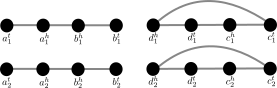
\includegraphics[width=0.9\textwidth]{figures/perfectly_duplicated_genomes.pdf}
% 		\end{center}
% 	\end{minipage}
% 	\begin{minipage}[b]{0.48\textwidth}
% 		\begin{center}
% 			\includegraphics[width=0.9\textwidth]{figures/duplicated_genomes.pdf}
% 		\end{center}
% 	\end{minipage}
% 		\caption{Left: Genome graph of perfectly duplicated genome $G \oplus
% 		G=\{\{a_1^t,\circ\},\{a_1^h,b_1^h\},\{b_1^t,\circ\},
% 		\{c_1^t,d_1^h\},\{d_1^t,c_1^h\},\{a_2^t,\circ\},\{a_2^h,b_2^h\},\{b_2^t,\circ\},
% 		\{c_2^t,d_2^h\},\{d_2^t,c_2^h\}\}$ where $G$ is defined in
% 		\Cref{fig:genome_graph}. Right: An example for a duplicated Genome
% 		$\Pi=\{\{a_1^t,\circ\},\{a_1^h,b_1^h\},\{b_1^t,c_1^h \},\{c_1^t,d_1^h \},
% 		\{d_1^t,b_2^t \},\{b_2^h,a_2^h \},\{a_2^t,\circ\},\{d_2^h,\circ\}, 
% 		\{d_2^t,c_2^h\}, \{c_2^t,\circ\} \}$. Note that a duplicated genome 
% 		can be seen as a rearranged perfectly duplicated genome.}
% 		\label{fig:duplicated_genomes}
% \end{figure}
% 
% %%%%%%%%%%%%%%%%%%%%%%% double distance %%%%%%%%%%%%%%%%%%%%%%%%%%%%
% The distance problem was also studied for the case of duplicated genomes, where
% under a specific model the minimum number of events to rearrange a perfectly
% duplicated genome $G \oplus G$ into a duplicated genome $\Pi$ is of interest.
% %
% This problem is referred as \emph{double distance problem}.
% %
% Equally to the distance problem, the double distance of a perfectly duplicated
% genome $G \oplus G$ and a duplicated genome $\Pi$ under a model $\m{M}$ is
% denoted by $d_\mathcal{M}(G
% \oplus G,\Pi)=\min_{S\in\m{S}^\m{M}_{(G \oplus G,\Pi)}}|\{S\}|$.
% %
% \re{FACTS ABOUT DD problem}
% 
% %%%%%%%%%%%%%%%%%%%%%%% halving %%%%%%%%%%%%%%%%%%%%%%%%%%%%
% Given a duplicated genome $\Pi$ and a model $\m{M}$ the \emph{halving problem}
% asks for a perfectly duplicated genome $G \oplus G$ such that the double
% distance between $\Pi$ and $G\oplus G$ under $\m{M}$ is minimized, i.e., the
% problem is to find $G \in \mathbb{G}$ which solves $\min_{G \in \mathbb{G}}
% d_{\m{M}}(\Pi,G \oplus G)$.
% %
% Note that the halving problem aims for finding a perfectly duplicated genome
% which might be the result of a whole duplication event and therefore it allows
% inference about parsimonious ancestor genomes before whole genome duplication
% events~\cite{Tannier_2008}.
% 
% %%%%%%%%%%%%%%%%%%%%%%% guided halving %%%%%%%%%%%%%%%%%%%%%%%%%%%%
% A recently presented \re{CITE} alternative of halving problem is the
% \emph{guided halving problem}.
% %
% If a duplicated genome $\Pi$ and a genome $\Gamma$ are presumed to share a
% common ancestor the halving problem can be guided such that the aim is to find a
% genome $G$ which comparably minimizes the distance $d_{\m{M}}(G,\Gamma)$ and the
% double distance $d_{\m{M}}(G \oplus G, \Pi)$.
% %
% Thus, for given $\Pi$, $\Gamma$, and $\m{M}$ the guided halving problem is to
% find a genome $G$ which satisfies $\min_{G \in \mathbb{G}} d_{\m{M}}(G,\Gamma)
% + d_{\m{M}}(G \oplus G, \Pi)$.
% 
% %%%%%%%%%%%%%%%%%%%%%%% aliquoting %%%%%%%%%%%%%%%%%%%%%%%%%%%%
% Note that \re{AUTHORS} presented in \re{CITE} a generalization of the halving
% problem for $n$-times copied genomes, which contain every gene exactly $n$
% times.
% %
% Due to limited space the so-called genome \emph{aliquoting problem} is not
% discussed in this chapter.
% %
% Interested readers should see \re{CITE} for an overview.
% 
% %%%%%%%%%%%%%%%%%%%%%%% natural graph %%%%%%%%%%%%%%%%%%%%%%%%%%%%
% In the present of a duplicated genomes with regard to halving problems the
% relationship between paralogous extremities are important, since they make the 
% difference between duplicated and perfectly duplicated genomes.
% %
% To represent the relations between paralogous extremities El-Mabrouk presented
% in~\cite{El-Mabrouk_2003} the \emph{natural graph}.
% %
% For a duplicated genome the natural graph contains all adjacencies as
% vertices which are connected by an undirected edges if and only if both
% adjacencies share a paralogous extremity.
% %
% Thus, for a duplicated genome $\Pi$ the natural graph is
% defined by $NG(\Pi):=G(V,E)$ where $V=\Pi$ and $E=\{(u,v): \exists u:=\{p,q\}\in
% \Pi \text{ and } v:=\{r,s\} \in \Pi: p=\hat{r} \text{ or } p=\hat{q}\}$.
% %
% \Cref{fig:natural_genome_example} illustrates the natural graph of the
% duplicated genome $\Pi$ defined in \Cref{fig:duplicated_genomes}.
% %
% \begin{figure}[htmb]
% 		\begin{minipage}[b]{0.9\textwidth}
% 			\begin{center}
% 				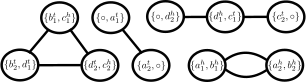
\includegraphics[width=.5\textwidth]{figures/natural_graph_example.pdf}
% 			\end{center}
% 		\end{minipage}
% 		\caption{Natural graph $NG(\Pi)$ of duplicated genome $\Pi$ as in
% 		\Cref{fig:duplicated_genomes}. $NG(\Pi)$ consists, respectively from left side
% 		to right side, of one odd cycle, one odd path, one even path, and one even
% 		cycle.}
% 		\label{fig:natural_genome_example}
% \end{figure}
% %
% Since every adjacency consists of two or one extremities, every vertex of the
% natural graph has degree of at most two.
% % (0 -> \{p,\hat{p}\}, 1 -> \{\circ, p\}, 2 -> \{p,q\} with p \neq \hat{q})
% %
% Thus, the natural graph is an union of cycles and paths which are distinguished
% into \emph{odd cycles}, \emph{even cycles}, \emph{odd paths}, and
% \emph{even paths} based on the number of edges they contain.
% %
% 
% %%%%%%%%%%%%%%%%%%%%%%% SCOJ %%%%%%%%%%%%%%%%%%%%%%%%%%%%
% %halving problem
% In~\cite{Feijao_2009} a similar strategy (like genome median problem) based on
% the fact that the cost of inclusion or exclusion of every adjacency in the searched genome is used
% to solve the (guided) genome halving problem in polynomial time such that 
% the constructed solution is unique.
% %
% %For a given duplicated genome $\Pi$ an adjacency $\{x,y\}$ is choosed as
% %adjacency of $G$ if and only if $2-2|\{ \{x_i,y_j\} \in \Pi: i,j \in [1:2]\}| <
% %0$.
% %
% 
% %%%%%%%%%%%%%%%%%%%%%%% DCJ %%%%%%%%%%%%%%%%%%%%%%%%%%%%
% %%%%%%%%%%%%%HALVING PROBLEM%%%%%%%%%%%%%%%%%%%%%%%%%
% The halving problem under the $\m{DCJ}$ model was studied in
%~\cite{Mixtacki_2008,Warren_2009} resulting linear time algorithms
% for the construction of the halving.
% %
% The model considered in~\cite{Mixtacki_2008} differs from the
% model considered in~\cite{Warren_2009} in the fact that single linear chromosome
% halving are prohibited by not allowing adjacencies of the form $\{q,\hat{q}\}$.
% %
% On the one hand this specialization prohibits linear single chromosome halvings
% and leads to an algorithm which works directly on the natural graph which is not
% the case in the algorithm presented in~\cite{Warren_2009} where complicated
% components of the breakpoint graph can be ignored by allowing single chromosome
% halvings.
% %
% On the other hand, circular single chromosome halvings are prohibited as
% well in~\cite{Mixtacki_2008} which is not the case in other papers on genome
% halving~\cite{Alekseyev_2007b,El-Mabrouk_2003} further examples with
% single circular chromosome halvings containing $\{q,\hat{q}\}$ which have a
% smaller distance than single circular chromosome halvings without adjacencies of
% this form are not covered by the model presented by Mixtacki.
% %
% 
% \re{Check genome halving, i understood sth wrong for example d(a,b) or d(b,a)}
% In~\cite{Mixtacki_2008} the reconstruction of a perfectly duplicated genome $G
% \oplus G$ for a duplicated genome $\Pi$ is done in three main steps.
% %
% The first step is the reconstruction of the natural graph $NG(\Pi)$ followed by
% maximizing the number of even cycles and odd paths in the natural graph.
% %
% Finally, the perfectly duplicated genome is reconstructed by the resulting
% natural graph.
% %
% The second step of maximizing even cycles and odd paths in $NG(\Pi)$ is based on
% the fact that the natural graph of a perfectly duplicated genome on the same
% set of genes of $\Pi$ with maximum number of even cycles and odd paths has the
% minimum distance to $\pi$, i.e., $min_{G \in \mathbb{G}} d_{\m{DCJ}}(\Pi,G\oplus
% G)= N - ( |EC| + \lfloor |OP| /2 \rfloor )$ where $|EC|$ and $|OP|$ is the
% number of even cycles and the number of odd paths, respectively.
% %
% See~\cite{Mixtacki_2008} for detailed proof. 
% %
% All three steps can be implemented in linear time as described in
%~\cite{Mixtacki_2008}.
% 
% In contrast to the algorithm presented by Mixtacki, the reconstruction algorithm
% presented by Warren and Sankoff calculates the independent set of $NG(\Pi)$
% \re{(which can be done in linear time for natural graphs since every vertex has
% degree of at most two)} after the construction of $NG(\Pi)$.
% %
% The perfectly duplicated genome $G\oplus G$ is derived from the independent set 
% by including $\{p,q\}\cup\{\hat{p},\hat{q}\}$ in $G\oplus G$ for every
% adjacency $\{p,q\}$ contained in a vertex of $NG(\Pi)$.
% %
% See~\cite{Warren_2009} for a detailed description.
% 
% %
% In the following we will shortly mention other polynomial time algorithms due to
% space limitations. 
% % DCJ + Indel operations for genomes with unequal gene content but
% % without duplicated genes
% Braga et al. presented in~\cite{Braga_2010,Braga_2011} a
% linear time algorithm for solving the sorting problem for multichromosomal
% genomes with unequal gene content but without duplicated genes.
% %
% For this so-called indel operations which allow the deletion and insertion of
% genes are added to the $\m{DCJ}$ model.
% %
% Recently Braga and Stoye presented in~\cite{Braga_2015} an $O(n \log{n})$
% algorithm which exactly solves the sorting problem for multichromosomal
% genomes with linear chromosomes only and unequal gene content but without
% duplicated genes.
% 
% Further~\cite{Tannier_2009} proved the NP-hardness of the double distance problem
% under $\m{DCJ}$ and the guided halving problem under the $\m{DCJ}$ model by
% a proof based on~\cite{Caprara_2003} and by reduction from BGD, respectively.
% 
% % duplicated genes %
% So far all presented algorithms assume that a genome contain either no
% duplicated genes or every gene exactly two times.
% %
% However, the principle of duplication is well-excepted as a major force of
% evolution~\cite{Ohno_2013}.
% %
% Therefor the distance problem for genomes with duplicated genes under the
% $\m{DCJ}$ model with indel operations was studied in~\cite{Shao_2012,Shao_2014}.
% %
% This problem turned out to be NP-hard as well~\cite{Shao_2014}.
% %
% While~\cite{Shao_2012} presents a heuristic which is based on finding the
% maximum number of certain cycles Shao et al.
% presented in~\cite{Shao_2014} an inter linear program which solves the distance problem for genomes with duplicated genes under the
% $\m{DCJ}$ model with indel operations exactly.
% %

%%%%%%%%%%%%%%%%%%%%%%% conclusion %%%%%%%%%%%%%%%%%%%%%%%%%%%%
\section{Conclusion}
\label{Sec-Concl}

In this chapter we have given an overview on genome rearrangement analysis. The focus was on the following two approaches. 
The first approach is the development of models for rearrangement mutations that are well suited for a theoretical analysis. 
In particular, models that use the two operations cut, i.e., to split a chromosome into fragments, and join, i.e., to merge 
fragments of chromosomes to new chromosomes. The second approach is to identify biologically motivated constraints on the 
applicability of gene rearrangement mutations. In particular, constraints that model conserved gene clusters have been 
considered. Several open problems for genome rearrangement analysis have been mentioned.


%
%Two approaches for genome rearrangement analysis that circumvent the difficulties caused by the incorporation of multiple types of genome rearrangement analysis
%have been presented.
%This is in particular the transposition operation,
%the absence of the information on the strandedness of the genes, 
%duplicated genes, and genomes with different gene content
%(where the later ones have not been discussed here, see
%\cite{Braga_2011,Shao_2014,Warren_2009,Yancopoulos_2008} and references) 
%which causes problems which are otherwise easily solvable to become intractable.
%
%A simplification of the problems is achieved by generalized models that are
%based on the cut and/or join of adjacencies and gene cluster preserving
%rearrangement analysis. Both simplify the core problems of rearrangement analysis, i.e., sorting,
%distance, median, and small phylogeny. 

\bibliographystyle{spmpsci}
\bibliography{dcj_overview}
 
\end{document}
